\ifdefined \buildingFullOPALManual \else


%\ifx \@buildingFullOPALManual \@empty
%\else

%\documentclass[12pt,a4paper]{report}
\documentclass[a4paper]{book}

%% does not work in Latex2Html mode
%\usepackage{hyperref}

\usepackage[T1]{fontenc}
\usepackage{url}
\usepackage{html}
\usepackage{epic}
\usepackage{eepic}
\usepackage{makeidx}
\usepackage{array}
\usepackage{times}
\usepackage{amsmath}
\usepackage{amsxtra}
\usepackage{bm}
\usepackage[thin,thinp,thinc]{esdiff}
\usepackage{graphicx}
\usepackage{dingbat}
\usepackage{color}
\usepackage{subfig}
\usepackage{boxedminipage}
\usepackage{alltt}
\usepackage{nicefrac}
\usepackage{calc}
%\usepackage{pdfdraftcopy}             % Draft
\usepackage{tikz}
\usetikzlibrary{
  er,3d,calc,fadings,trees,positioning,arrows,chains,decorations.pathreplacing,
  decorations.pathmorphing,shapes,shapes.symbols,shapes.arrows,matrix,through,decorations.text
}

\tikzset{
  >=stealth',
  punktchain/.style={rectangle,rounded corners, draw=black, very thick,text width=10em,
                     minimum height=3em, text centered, on chain},
  line/.style={draw, thick, <-},
  element/.style={tape,top color=white,bottom color=blue!50!black!60!,minimum width=8em,
                  draw=blue!40!black!90, very thick,text width=10em, minimum height=3.5em,
                  text centered, on chain},
  every join/.style={->, thick,shorten >=1pt},
  tuborg/.style={decorate},
  tubnode/.style={midway, right=2pt}
}

\tikzstyle{material}=[draw, fill=blue!20, text width=16.0em, text centered, minimum height=1.5em]
\tikzstyle{diagramstep} = [material, text width=20em, minimum width=10em, minimum height=3em, rounded corners]
\tikzstyle{line} = [draw, thick, color=black!50, -latex']

\usepackage{booktabs}
\usepackage{xspace}
\usepackage{xstring}

\usepackage{fancyvrb}
\usepackage{rotating}
\usepackage{float}

\usepackage{tabularx}
\usepackage{longtable}
\setcounter{LTchunksize}{3}

\usepackage[section]{placeins}
\usepackage{MnSymbol}
\usepackage{microtype}
\usepackage{setspace}
\usepackage{dcolumn}

\usepackage[vmargin={3.0cm,3.0cm},
            hmargin={2.0cm,3.0cm}]{geometry}

\usepackage{upgreek}
\usepackage[binary-units=true]{siunitx}
\sisetup{exponent-product = \cdot,math-ohm=\Upomega,text-ohm=\ensuremath{\Upomega}}
\DeclareSIUnit{\clight}{c}
\DeclareSIUnit\gauss{Ga}

\usepackage{engord}
\usepackage{wasysym}
\DeclareSIUnit[number-unit-product = \,]{\permill}{\permil}

\usepackage{hyperref}
\hypersetup{
    pdftitle          = The OPAL Framework,
    pdfauthor         = {Andreas Adelmann, Achim Gsell, Valeria Rizzoglio, Christof Metzger-Kraus,
                         Yves Ineichen, Xiaoying Pang, Steve Russell, Chuan Wang, Jianjun Yang,
                         Suzanne Sheehy, Chris Rogers, Daniel Winklehner},
    pdfsubject        = User's Reference Manual,
    pdffitwindow      = true,               % page fit to window when opened
    pdfnewwindow      = true,               % links in new window
    colorlinks        = true,               % false: boxed links; true: colored links
    linkcolor         = black!80!green,     % color of internal links
    citecolor         = black!20!red,       % color of links to bibliography
    urlcolor          = blue,               % color of external links
    breaklinks        = true,
    bookmarksnumbered = true,
    plainpages        = false
}

\usepackage{ifthen}

\newif \iflinuxwindows
\linuxwindowstrue   % set this to true when building the manual on Linux or Windows
\iflinuxwindows
\usepackage{epstopdf}
\fi

\usepackage[backend=biber,
            style=phys,
            biblabel=brackets,
            maxnames=3,
            doi=true,
            isbn=true,
            url=true]{biblatex}
%---- macros ----

\renewcommand{\topfraction}{1.0}
\renewcommand{\bottomfraction}{1.0}
\renewcommand{\textfraction}{0.0}
\renewcommand{\arraystretch}{2.0}
\newenvironment{tex2html_nowrap}{}{}


\newcommand{\Newline}{\hfil \\}


\newsavebox{\ExampleBox}
\newenvironment{example}
 {\VerbatimEnvironment
  \begin{flushleft}
  \begin{lrbox}{\ExampleBox}
    \begin{minipage}{\linewidth}
  \begin{Verbatim}[frame=lines,xleftmargin=0cm,fontsize=\footnotesize,samepage=true]}
 {\end{Verbatim}
  \end{minipage}
  \end{lrbox}
  \mbox{\usebox{\ExampleBox}}
  \end{flushleft}
 }

\newenvironment{longexample}
{\Verbatim[frame=lines,xleftmargin=0mm,fontsize=\footnotesize]}
{\endVerbatim}

%\examplefromfile{filename} reads in a text file and displays it in the document.
\newcommand{\examplefromfile}[1]{
\VerbatimInput[frame=lines,xleftmargin=0mm,fontsize=\footnotesize,label=\texttt{#1}]{#1}}

%for upright d of differentials
\makeatletter
\newcount\my@repeat@count

\newcommand{\myrepeat}[2]{%
  \begingroup
  \my@repeat@count=\z@
  \@whilenum\my@repeat@count<#1\do{#2\advance\my@repeat@count\@ne}%
  \endgroup
}

\newcommand{\differential}[1]{\ifstrempty{#1}{\ES@dop\ES@difint}{\ES@dop^{#1}\ES@difint}}
\newcommand{\pdifferential}[1]{\ifstrempty{#1}{{\partial\,}}{{\partial^{#1}\,}}}

\makeatother

\newcommand{\der}[3][]{\frac{\differential{#1}#2}{\differential{}\ifstrempty{#1}{#3}{#3^#1}}}
\newcommand{\parder}[3][]{\frac{\pdifferential{#1}#2}{\pdifferential{}\ifstrempty{#1}{#3}{#3^#1}}}
\newcommand{\niceder}[3][]{\nicefrac{\differential{#1}#2}{\differential{}\ifstrempty{#1}{#3}{#3^#1}}}
\newcommand{\uglyder}[3][]{{\differential{#1}#2}/{\differential{}\ifstrempty{#1}{#3}{#3^#1}}}
\newcommand{\uglyparder}[3][]{{\pdifferential{#1}#2}/{\pdifferential{}\ifstrempty{#1}{#3}{#3^#1}}}
\newcommand{\dd}[1][]{\; \differential{#1}}
\newcommand{\primed}{^{\prime}}
\newcommand{\dprimed}{^{\prime\prime}}
\newcommand{\nprimed}[1]{^{\myrepeat{#1}{\prime}}}

%Editing Macros
\newcommand{\TODO}[1]{{\color{red}\ifthenelse{\boolean{ShowDebug}}{[TODO: #1]}{}}}



%text in gray box
\newsavebox{\fmbox}
\definecolor{lightgray}{gray}{0.95}
\newenvironment{fmpage}
   {\vspace{-1.0cm}\begin{lrbox}{\fmbox}\begin{minipage}[t]{13.5cm}\vspace{0.1cm}}
   {\vspace{-0.4cm}\end{minipage}\end{lrbox}\begin{center}\fcolorbox{black}{lightgray}{\usebox{\fmbox}}\end{center}}


% Definition new signes
\newcommand{\R}{{\mathbb R}} % real numbers
\newcommand{\Q}{{\mathbb Q}} % rational numbers
\newcommand{\Z}{{\mathbb Z}} % integer numbers
\newcommand{\N}{{\mathbb N}} % natural numbers

\newcommand{\mad}{\textsc{mad}\xspace}
\newcommand{\madnine}{\textsc{mad9}\xspace}
\newcommand{\madninep}{\textsc{mad9p}\xspace}
\newcommand{\madeight}{\textsc{mad8}\xspace}
\newcommand{\classic}{\textsc{classic}\xspace}

\makeatletter
\newcommand{\opal@impl}{\textsc{Opal}}
\newcommand{\opalt@impl}{\textsc{Opal-t}}
\newcommand{\opalcycl@impl}{\textsc{Opal-cycl}}
\newcommand{\opalmap@impl}{\textsc{Opal-map}}
\newcommand{\opalenv@impl}{\textsc{Opal-e}}

\newcommand{\opal}{\opal@impl\xspace}
\newcommand{\opalt}{\opalt@impl\xspace}
\newcommand{\opalcycl}{\opalcycl@impl\xspace}
\newcommand{\opalmap}{\opalmap@impl\xspace}
\newcommand{\opalenv}{\opalenv@impl\xspace}

\newcommand{\noopalt}{\leftthumbsdown \opalt@impl\xspace}
\newcommand{\noopalcycl}{\leftthumbsdown \opalcycl@impl\xspace}
\newcommand{\noopalmap}{\leftthumbsdown \opalmap@impl\xspace}
\newcommand{\noopalenv}{\leftthumbsdown \opalenv@impl\xspace}
\makeatother

\newcommand{\impactt}{\textsc{Impact-t}\xspace}
\newcommand{\partroot}{\textsc{H5root}}


\newcommand{\latermore}{More details will be given in Version 1.6.0}


\newcommand{\lieop}[1]{{:}{#1}{:}}

\newcommand{\rms}[1]{\overset{\sim}{#1}}

\newcommand{\sprod}{\cdot}
\newcommand{\vprod}{\times}
\newcommand{\matr}[1]{\mathcal{#1}}
\renewcommand{\vec}[1]{{\bm{#1}}}
\newcommand{\transpose}[1]{#1^\intercal}
\renewcommand{\epsilon}{\varepsilon}

\newcommand{\keyword}[2][]{\ifstrempty{#1}{\texttt{\expandafter\MakeUppercase\expandafter{#2}}}{\hyperref[#1]{\texttt{\expandafter\MakeUppercase\expandafter{#2}}}}}
\newcommand{\tabline}[3][]{\keyword[#1]{#2}& #3 \\}
\newcommand{\tabheadcell}[1]{{\bfseries #1}}

\newcommand*\kdescriptionlabel[1]{\hspace\labelsep
                                \normalfont\keyword{#1}\index{#1}}
\makeatletter
\newenvironment{kdescription}
               {\list{}{\labelwidth\z@ \itemindent-\leftmargin
                        \let\makelabel\kdescriptionlabel}}
               {\endlist}
\makeatother

\ExplSyntaxOn
\NewDocumentCommand{\tabhead}{ m }
 {
  \seq_set_split:Nnn \l_tmpa_seq { & } { #1 }
  \bfseries \seq_use:Nn \l_tmpa_seq { & \bfseries } \\
 }

\NewDocumentCommand \multrefImpl { O{ } m m m } {
  \ifnumgreater{\clist_count:n {#4}}{1}{
    \seq_set_from_clist:Nn \l_tmpa_seq { #4 }

    \seq_set_map:NNn \l_tmpb_seq \l_tmpa_seq { \exp_not:n { \ref{#3:##1} } }
    \ifstrempty{#1}{#2s}{#1}~\seq_use:Nnnn \l_tmpb_seq {\ and\ } {,\ } {,\ and\ }
  }{
    #2~\ref{#3:#4}
  }
}

\NewDocumentCommand \multeqnrefImpl { m } {
  \ifnumgreater{\clist_count:n {#1}}{1}{
    \seq_set_from_clist:Nn \l_tmpa_seq { #1 }

    \seq_set_map:NNn \l_tmpb_seq \l_tmpa_seq { \exp_not:n { \eqref{eq:##1} } }
    Equations~\seq_use:Nnnn \l_tmpb_seq {\ and\ } {,\ } {,\ and\ }
  }{
    Equation~\eqref{eq:#1}
  }
}
\ExplSyntaxOff


%Abbreviations for Equations, Figures, and Tables
%\newcommand{\Equation}[1]{Equation~\eqref{#1}}

\newcommand{\bibref}[2]{#1 \cite{bib:#2}}
\newcommand{\figref}[1]{\multrefImpl{Figure}{fig}{#1}}
\newcommand{\chpref}[1]{\multrefImpl{Chapter}{chp}{#1}}
\newcommand{\appref}[1]{\multrefImpl[Appendices]{Appendix}{chp}{#1}}
\newcommand{\secref}[1]{\multrefImpl{Section}{sec}{#1}}
\newcommand{\ssecref}[1]{\multrefImpl{Section}{ssec}{#1}}
\newcommand{\tabref}[1]{\multrefImpl{Table}{tab}{#1}}
\newcommand{\eqnref}[1]{\multeqnrefImpl{#1}}

\newcommand{\seefig}[1]{(see~\figref{#1})}
\newcommand{\seechp}[1]{(see~\chpref{#1})}
\newcommand{\seesec}[1]{(see~\secref{#1})}
\newcommand{\seessec}[1]{(see~\ssecref{#1})}
\newcommand{\seetab}[1]{(see~\tabref{#1})}
\newcommand{\seeeqn}[1]{(see~\eqnref{#1})}

\newcommand{\filename}[1]{\emph{#1}}


% Define distances for bordering
\newcommand{\blockdist}{1.3}
\newcommand{\edgedist}{1.5}
\newcommand{\diagramstep}[2]{node (p#1) [diagramstep] {#2}}


% place chapter title page on odd pages
\let\stdchapter\chapter
\makeatletter
\renewcommand*{\chapter}{\if@openright\cleardoublepage\else\clearpage\fi\stdchapter}

\makeatother

\IfFileExists{./version.tex}{%
  \newcommand{\opalversion}[1]{Version \ifstrempty{#1}{1.9.0}{#1}\xspace}
%
}%
{%
  \newcommand{\opalversion}[1]{\ifstrempty{#1}{current Version}{Version #1}\xspace}%
}
\newboolean{ShowMap}
\setboolean{ShowMap}{false}

\newboolean{ShowEnv}
\setboolean{ShowEnv}{false}

\newboolean{ShowDebug}
\setboolean{ShowDebug}{false}

%----Control Structures
\newboolean{FullOPALManual}
\setboolean{FullOPALManual}{false}


\makeindex


\bibliography{bibliography}
\begin{document}

\fi

\chapter{Elements}
\label{chp:element}
\index{Elements|(}

\section{Element Input Format}
\label{sec:elm-format}
\index{Element!Format}
All physical elements are defined by statements of the form
\begin{example}
label:keyword, attribute,..., attribute
\end{example}
where
\begin{description}

\item[label]
  \index{Element!Label} \Newline
  Is the name to be given to the element (in the example QF),
  it is an {identifier} \seesec{label}.

\item[keyword] \Newline
  \index{Element!Keyword}
  Is a {keyword} \seesec{label},
  it is an element type keyword (in the example \keyword{QUADRUPOLE}),
\item[attribute]  \Newline
  \index{Element!Attribute}
  normally has the form
\begin{example}
attribute-name=attribute-value
\end{example}
\item[attribute-name]  \Newline
  selects the attribute from the list defined for the element type
  \texttt{keyword} (in the example \keyword{L} and \keyword{K1}).
  It must be an {identifier} \seesec{label}
\item[attribute-value] \Newline
  gives it a {value} \seesec{attribute}
  (in the example \texttt{1.8} and \texttt{0.015832}).
\end{description}
Omitted attributes are assigned a default value, normally zero.

\noindent Example:
\begin{example}
QF: QUADRUPOLE, L=1.8, K1=0.015832;
\end{example}



\section{Common Attributes for all Elements}
\label{sec:Element:common}
\index{Element!Common Attributes}
The following attributes are allowed on all elements:
\begin{kdescription}
\item[TYPE]
  A {string value} \seesec{astring}.
  It specifies an ``engineering type'' and can be used for element
  selection.
\item[APERTURE]
  A {string value} \seesec{astring} which describes
  the element aperture.
  All but the last attribute of the aperture have units of meter, the last one is optional and is a positive real number. Possible choices are
  \begin{itemize}
  \item \texttt{APERTURE}="\texttt{SQUARE}(\texttt{a,f})" has a square shape of width and height \texttt{a},
  \item \texttt{APERTURE}="\texttt{RECTANGLE}(\texttt{a,b,f})" has a rectangular shape of width \texttt{a} and height \texttt{b},
  \item \texttt{APERTURE}="\texttt{CIRCLE}(\texttt{d,f})" has a circular shape of diameter \texttt{d},
  \item \texttt{APERTURE}="\texttt{ELLIPSE}(\texttt{a,b,f})" has an elliptical shape of major \texttt{a} and minor \texttt{b}.
  \end{itemize}
  The option \texttt{SQUARE}(\texttt{a,f}) is equivalent to \texttt{RECTANGLE}(\texttt{a,a,f}) and \texttt{CIRCLE}(\texttt{d,f}) is equivalent to \texttt{ELLIPSE}(\texttt{d,d,f}). The size of the exit aperture is scaled by a factor $f$. For $f < 1$ the exit aperture is smaller than the entrance aperture, for $f = 1$ they are the same and for $f > 1$ the exit aperture is bigger.

  Dipoles have \keyword{GAP} and \keyword{HGAP} which define an aperture and hence do not recognise \keyword{APERTURE}. The aperture of the dipoles has rectangular shape of height \keyword{GAP} and width \keyword{HGAP}. In longitudinal direction it is bent such that its center coincides with the circular segment of the reference particle when ignoring fringe fields. Between the beginning of the fringe field and the entrance face and between the exit face and the end of the exit fringe field the rectangular shape has width and height that are twice of what they are inside the dipole.

  Default aperture for all other elements is a circle of \SI{1.0}{\meter}.

\item[L]
  The length of the element (default: \SI{0}{\meter}).
\item[WAKEF]
  Attach wakefield that was defined using the \keyword[sec:wakecmd]{WAKE} command.
\item[ELEMEDGE]
    The edge of an element is specified in s coordinates in meters. This edge corresponds to the origin of the local coordinate system and is the physical start of the element. (Note that in general the fields will extend in front of this position.) The physical end of the element is determined by \keyword{ELEMEDGE} and its physical length. (Note again that in general the fields will extend past the physical end of the element.)
\item[PARTICLEMATTERINTERACTION]
  Attach a handler for particle matter interaction, see \ref{chp:partmatt}.
\item[X]
  X-component of the position of the element in the laboratory coordinate system.
\item[Y]
  Y-component of the position of the element in the laboratory coordinate system.
\item[Z]
  Z-component of the position of the element in the laboratory coordinate system.
\item[THETA]
  Angle of rotation of the element about the y-axis relative to the default orientation, $\vec{n} = \transpose{\left(0, 0, 1\right)}$.
\item[PHI]
  Angle of rotation of the element about the x-axis relative to the default orientation, $\vec{n} = \transpose{\left(0, 0, 1\right)}$ \item[PSI]
  Angle of rotation of the element about the z-axis relative to the default orientation, $\vec{n} = \transpose{\left(0, 0, 1\right)}$ \item[ORIGIN]
  3D position vector. An alternative to using \keyword{X}, \keyword{Y} and \keyword{Z} to position the element. Can't be combined with \keyword{THETA} and \keyword{PHI}. Use \keyword{ORIENTATION} instead.
\item[ORIENTATION]
  Vector of Tait-Bryan angles \cite{bib:tait-bryan}. An alternative to rotate the element instead of using \keyword{THETA}, \keyword{PHI} and \keyword{PSI}. Can't be combined with \keyword{X}, \keyword{Y} and \keyword{Z}, use \keyword{ORIGIN} instead.
\item[DX]
  Error on x-component of position of element. Doesn't affect the design trajectory.
\item[DY]
  Error on y-component of position of element. Doesn't affect the design trajectory.
\item[DZ]
  Error on z-component of position of element. Doesn't affect the design trajectory.
\item[DTHETA]
  Error on angle \keyword{THETA}. Doesn't affect the design trajectory.
\item[DPHI]
  Error on angle \keyword{PHI}. Doesn't affect the design trajectory.
\item[DPSI]
  Error on angle \keyword{PSI}. Doesn't affect the design trajectory.

\end{kdescription}

All elements can have arbitrary additional attributes which are defined in the respective section.

\clearpage

\section{Drift Spaces}
\label{sec:drift}
\index{DRIFT}
\begin{example}
label:DRIFT, TYPE=string, APERTURE=string, L=real;
\end{example}
A DRIFT space has no additional attributes.
\noindent Examples:
\begin{example}
DR1:DRIFT, L=1.5;
DR2:DRIFT, L=DR1->L, TYPE=DRF;
\end{example}
The length of \texttt{DR2} will always be equal to the length of \texttt{DR1}.
The reference system for a drift space is a Cartesian coordinate system
\ifthenelse{\boolean{ShowMap}}{\seefig{straight}}{}.
This is a restricted feature: \noopalcycl. In \opalt drifts are implicitly given, if no field is present.



\clearpage
\section{Bending Magnets}
\label{sec:bend}
\index{Bending Magnets|(}
Bending magnets refer to dipole fields that bend particle trajectories. Currently \opal supports three different
bend elements: \keyword{RBEND}, (valid in \opalt, see \ssecref{RBend}), \keyword{SBEND} (valid in \opalt, see
\ssecref{SBend}), \keyword{RBEND3D}, (valid in \opalt, see \ssecref{RBend3D}) and \keyword{SBEND3D} (valid in
\opalcycl, see \ssecref{SBend3D}).

Describing a bending magnet can be somewhat complicated as there can be many parameters to consider: bend angle,
bend radius, entrance and exit angles etc. Therefore we have divided this section into several parts:

\begin{enumerate}
\item \ssecref{RBend,SBend} describe the geometry and attributes of the \opalt bend
  elements \keyword{RBEND} and \keyword{SBEND}.
\item \ssecref{RBendSBendExamp} describes how to implement an \keyword{RBEND} or \keyword{SBEND} in an
  \opalt simulation.
\item \ssecref{SBend3D} is self contained. It describes how to implement an \keyword{SBEND3D} element in
  an \opalcycl simulation.
\end{enumerate}

\begin{figure}[!htb]
  \begin{center}
    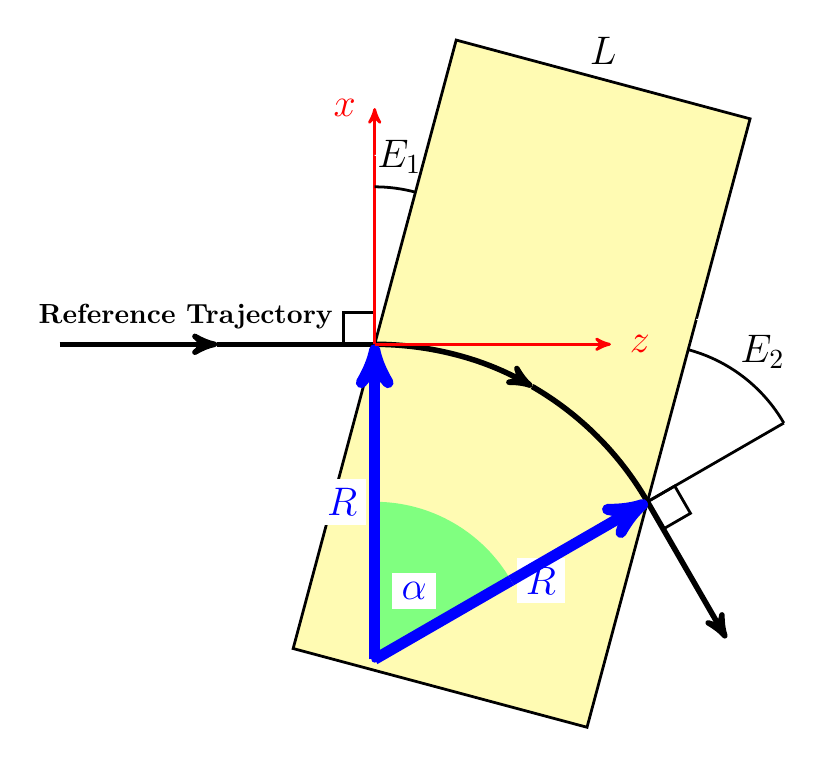
\begin{tikzpicture}[scale=4]
      % First draw rectangular magnet shape.
      \draw[white,rotate around={-15:(0.0,0.0)}] (0.0,1.0) -- (0.4829629,1.0)
      node[above=2pt] {\Large{\textbf{\color{black}$L$}}};
      \filldraw[yellow!30!white,rotate around={-15:(0.0,0.0)}] (0,-1.0) rectangle (0.9659258,1.0);
      \draw[line width=1pt,rotate around={-15:(0.0,0.0)}] (0,-1.0) rectangle (0.9659258,1.0);

      % Now draw squares indicating 90 degree angles to bend radius at entrance and exit.
      \draw[line width=1pt] (0.0,0.0) rectangle (-0.1,0.1);
      \draw[line width=1pt,rotate around={-60:(0.0,-1.0)}]
      (0.0,0.0) rectangle (0.1,0.1);

      % Draw reference particle path.
      \draw[white] (-1.1,0.0) -- (-0.6,0.0)
      node[above=2pt] {\textbf{\color{black}Reference Trajectory}};
      \draw[arrows=->,line width=2pt] (-1.0,0.0) -- (-0.5,0.0);
      \draw[line width=2pt] (-0.5,0.0) -- (0.0,0.0);
      \draw[arrows=->,line width=2pt] (0.0,0.0) arc (90:60:1.0);
      \draw[line width=2pt] (0.5,-0.133975) arc (60:30:1.0);
      \draw[arrows=->,line width=2pt] (0.8660254,-0.5) -- (1.1160254,-0.9330127);

      % Draw bend angle.
      \fill[green!50!white] (0.0,-1.0) -- (0.0,-0.5) arc (90:30:0.5) -- (0.0,-1.0);
      \draw[green!50!white] (0.0,-0.75) arc (90:60:0.25)
      node[fill=white] {\Large{\textbf{\color{blue}$\alpha$}}};

      % Draw bend radii at entrance and exit.
      \draw[blue,line width=4pt] (0.0,-1.0) -- (0.0,-0.5)
      node[blue,left=1pt,fill=white] {\Large{\textbf{$R$}}};
      \draw[arrows=->,blue,line width=4pt] (0.0,-0.5) -- (0.0,0.0);
      \draw[blue,line width=4pt] (0.0,-1.0) -- (0.4330127,-0.75)
      node[below=6pt,right=0pt,fill=white] {\Large{\textbf{$R$}}};
      \draw[arrows=->,blue,line width=4pt] (0.4330127,-0.75) -- (0.8660254,-0.5);
      \filldraw[blue] (0.0,-1.0) circle (0.25pt);

      % Draw reference axes.
      \draw[red,arrows=->,line width=1pt] (0.0,0.0) -- (0.0,0.75) node[left=3pt] {\Large{\textbf{$x$}}};
      \draw[red,arrows=->,line width=1pt] (0.0,0.0) -- (0.75,0.0) node[right=3pt] {\Large{\textbf{$z$}}};

      % Label entrance angle.
      \draw[line width=1pt] (0.0,0.5) arc (90:75:0.5);
      \draw[white] (0.0,0.6) arc (90:82.5:0.6) node[] {\Large{\textbf{\color{black}$E_{1}$}}};

      % Label exit angle.
      \draw[line width=1pt,xshift=0.8660254cm,yshift=-0.5cm,rotate around={-60:(0.0,0.0)}] (0.0,0.0) -- (0.0,0.5);
      \draw[line width=1pt,xshift=0.8660254cm,yshift=-0.5cm,rotate around={-15:(0.0,0.0)}] (0.0,0.5) arc(90:45:0.5);
      \draw[white,xshift=0.8660254cm,yshift=-0.5cm,rotate around={-15:(0.0,0.0)}] (0.0, 0.6) arc (90:67.5:0.6)
      node[] {\Large{\textbf{\color{black}$E_{2}$}}};

    \end{tikzpicture}
  \end{center}
  \caption{Illustration of a general rectangular bend (\keyword{RBEND}) with a positive bend angle $\alpha$. The
    entrance edge angle, $E_{1}$, is positive in this example. An \keyword{RBEND} has parallel entrance and exit
    pole faces, so the exit angle, $E_{2}$, is uniquely determined by the bend angle, $\alpha$, and $E_{1}$
    ($E_{2}=\alpha - E_{1}$). For a positively charge particle, the magnetic field is directed out of the page.}
  \label{fig:rbend}
\end{figure}

\subsection{RBend (\opalt)}
\label{ssec:RBend}
\index{RBEND}
An \keyword{RBEND} is a rectangular bending magnet. The key property of an \keyword{RBEND} is that is has parallel
pole faces. \figref{rbend} shows an \keyword{RBEND} with a positive bend angle and a positive entrance edge angle.

\begin{kdescription}
\item[L]
  Physical length of magnet (meters, see \figref{rbend}).

\item[GAP]
  Full vertical gap of the magnet (meters).

\item[HAPERT]
  Non-bend plane aperture of the magnet (meters). (Defaults to one half the bend radius.)

\item[ANGLE]
  Bend angle (radians). Field amplitude of bend will be adjusted to achieve this angle. (Note that for
  an \keyword{RBEND}, the bend angle must be less than $\nicefrac{\pi}{2} + E1$, where \keyword{E1} is the entrance edge angle.)

\item[K0]
  Field amplitude in y direction (Tesla). If the \keyword{ANGLE} attribute is set, \keyword{K0} is ignored.

\item[K0S]
  Field amplitude in x direction (Tesla). If the \keyword{ANGLE} attribute is set, \keyword{K0S} is ignored.

\item[K1]
  Field gradient index of the magnet, $K_1=-\frac{R}{B_{y}}\diffp{B_y}{x}$, where
  $R$ is the bend radius as defined in \figref{rbend}. Not supported in \noopalt any more. Superimpose a \keyword[sec:quadrupole]{Quadrupole} instead.

\item[E1]
  Entrance edge angle (radians). \figref{rbend} shows the definition of a positive entrance
  edge angle. (Note that the exit edge angle is fixed in an \keyword{RBEND} element to E2 = ANGLE
  $\text{\keyword{E2}} = \text{\keyword{ANGLE}} - \text{\keyword{E1}}$).

\item[DESIGNENERGY]
  Energy of the reference particle (\si{\mega\electronvolt}). The reference particle travels approximately the path shown in
  \figref{rbend}.

\item[FMAPFN]
  Name of the field map for the magnet. Currently maps of type \texttt{1DProfile1} can
  be used \seesec{1DProfile1}. The default option for this attribute is \keyword{FMAPN} =
  ``\keyword{1DPROFILE1-DEFAULT}'' \seessec{benddefaultfieldmapopalt}. The field map is used to
  describe the fringe fields of the magnet \seesec{1DProfile1}.

\end{kdescription}

\clearpage
\subsection{RBend3D (\opalt)}
\label{ssec:RBend3D}
\index{RBEND3D}
An \keyword{RBEND3D3D} is a rectangular bending magnet. The key property of an \keyword{RBEND3D} is that is has parallel
pole faces. \figref{rbend} shows an \keyword{RBEND3D} with a positive bend angle and a positive entrance edge angle.

\begin{kdescription}
\item[L]
  Physical length of magnet (meters, see \figref{rbend}).

\item[GAP]
  Full vertical gap of the magnet (meters).

\item[HAPERT]
  Non-bend plane aperture of the magnet (meters). (Defaults to one half the bend radius.)

\item[ANGLE]
  Bend angle (radians). Field amplitude of bend will be adjusted to achieve this angle. (Note that for
  an \keyword{RBEND3D}, the bend angle must be less than $\nicefrac{\pi}{2} + E1$, where \keyword{E1} is the entrance edge angle.)

\item[K0]
  Field amplitude in y direction (Tesla). If the \keyword{ANGLE} attribute is set, \keyword{K0} is ignored.

\item[K0S]
  Field amplitude in x direction (Tesla). If the \keyword{ANGLE} attribute is set, \keyword{K0S} is ignored.

\item[K1]
  Field gradient index of the magnet, $K_1=-\frac{R}{B_{y}}\diffp{B_y}{x}$, where
  $R$ is the bend radius as defined in \figref{rbend}. Not supported in \noopalt any more. Superimpose a \keyword[sec:quadrupole]{Quadrupole} instead.

\item[E1]
  Entrance edge angle (radians). \figref{rbend} shows the definition of a positive entrance
  edge angle. (Note that the exit edge angle is fixed in an \keyword{RBEND3D} element to E2 = ANGLE
  $\text{\keyword{E2}} = \text{\keyword{ANGLE}} - \text{\keyword{E1}}$).

\item[DESIGNENERGY]
  Energy of the reference particle (\si{\mega\electronvolt}). The reference particle travels approximately the path shown in
  \figref{rbend}.

\item[FMAPFN]
  Name of the field map for the magnet. Currently maps of type \texttt{1DProfile1} can
  be used \seesec{1DProfile1}. The default option for this attribute is \keyword{FMAPN} =
  ``\keyword{1DPROFILE1-DEFAULT}'' \seessec{benddefaultfieldmapopalt}. The field map is used to
  describe the fringe fields of the magnet \seesec{1DProfile1}.

\end{kdescription}
\clearpage

\begin{figure}[!htb]
  \begin{center}
    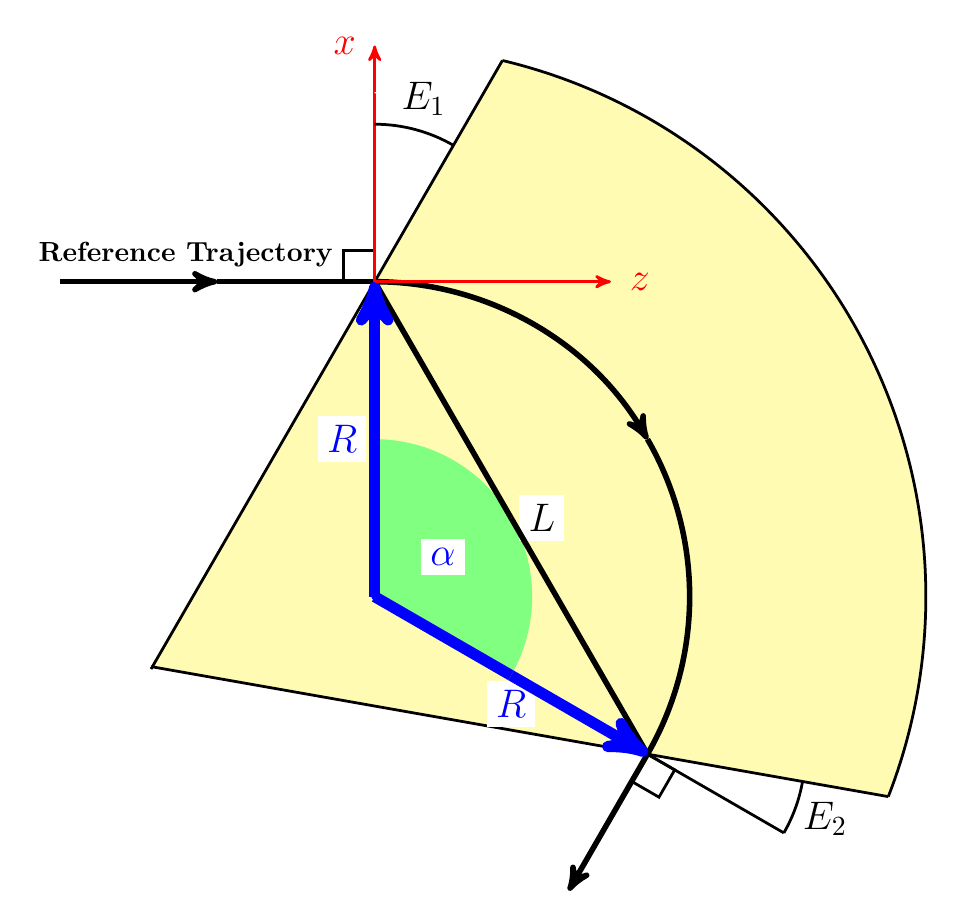
\begin{tikzpicture}[scale=4]
      % Draw magnet shape.
      \filldraw[yellow!30!white] (-0.709667,-1.22216292)
      -- (0.4055127895,0.702368754) arc (76.6015496:-21.2704331:1.75)
      -- (-0.709667,-1.22216292);

      \draw[line width=1pt, rotate around={-30:(0.0,0.0)}] (0,-1.42) -- (0,0.811025579);
      \draw[line width=1pt] (0.40551279,0.70236875) arc (76.6015496:-21.2704331:1.75);
      \draw[line width=1pt] (1.6307875,-1.6348482) -- (-0.709667,-1.22216292);

      % Now draw squares indicating 90 degree angles to bend radius at entrance and exit.
      \draw[line width=1pt] (0.0,0.0) rectangle (-0.1,0.1);
      \draw[line width=1pt,xshift=0.8660254cm,yshift=-1.5cm,rotate around={60:(0.0,0.0)}]
      (-0.1,-0.1) rectangle (0.0,0.0);

      % Draw reference particle path.
      \draw[white] (-1.1,0.0) -- (-0.6,0.0)
      node[above=2pt] {\textbf{\color{black}Reference Trajectory}};
      \draw[arrows=->,line width=2pt] (-1.0,0.0) -- (-0.5,0.0);
      \draw[line width=2pt] (-0.5,0.0) -- (0.0,0.0);
      \draw[arrows=->,line width=2pt] (0.0,0.0) arc (90:30:1.0);
      \draw[line width=2pt] (0.8660254,-0.5) arc (30:-30:1.0);
      \draw[arrows=->,line width=2pt] (0.8660254,-1.5) -- (0.6160254,-1.9330127);

      % Draw bend angle.
      \fill[green!50!white] (0.0,-1.0) -- (0.0,-0.5) arc (90:-30:0.5) -- (0.0,-1.0);
      \draw[green!50!white] (0.0,-0.75) arc (90:30:0.25)
      node[fill=white] {\Large{\textbf{\color{blue}$\alpha$}}};

      % Label chord length.
      \draw[line width=2pt] (0.0,0.0) -- (0.4330127,-0.75)
      node[fill=white,right=2pt] {\Large{\textbf{\color{black}$L$}}};
      \draw[line width=2pt] (0.4330127,-0.75) -- (0.8660254,-1.5);

      % Draw bend radii at entrance and exit.
      \draw[blue,line width=4pt] (0.0,-1.0) -- (0.0,-0.5)
      node[blue,left=1pt,fill=white] {\Large{\textbf{$R$}}};
      \draw[arrows=->,blue,line width=4pt] (0.0,-0.5) -- (0.0,0.0);

      \draw[blue,line width=4pt] (0.0,-1.0) -- (0.4330127,-1.25)
      node[below=0pt,fill=white] {\Large{\textbf{$R$}}};
      \draw[arrows=->,blue,line width=4pt] (0.4330127,-1.25) -- (0.8660254,-1.5);
      \filldraw[blue] (0.0,-1.0) circle (0.25pt);

     % Draw reference axes.
      \draw[red,arrows=->,line width=1pt] (0.0,0.0) -- (0.0,0.75) node[left=3pt] {\Large{\textbf{$x$}}};
      \draw[red,arrows=->,line width=1pt] (0.0,0.0) -- (0.75,0.0) node[right=3pt] {\Large{\textbf{$z$}}};

      % Label entrance angle.
      \draw[line width=1pt] (0.0,0.5) arc (90:60:0.5);
      \draw[white] (0.0,0.6) arc (90:75:0.6) node[] {\Large{\textbf{\color{black}$E_{1}$}}};

      % Label exit angle.
      \draw[line width=1pt,xshift=0.8660254cm,yshift=-1.5cm,rotate around={-120:(0.0,0.0)}] (0.0,0.0) -- (0.0,0.5);
      \draw[line width=1pt,xshift=0.8660254cm,yshift=-1.5cm,rotate around={-120:(0.0,0.0)}] (0.0,0.5) arc(90:110:0.5);
      \draw[white,xshift=0.8660254cm,yshift=-1.5cm,rotate around={-120:(0.0,0.0)}] (0.0, 0.6) arc (90:100:0.6)
      node[] {\Large{\textbf{\color{black}$E_{2}$}}};

    \end{tikzpicture}
  \end{center}
  \caption{Illustration of a general sector bend (\keyword{SBEND}) with a positive bend angle $\alpha$. In this example
    the entrance and exit edge angles $E_{1}$ and $E_{2}$ have positive values. For a positively charge particle,
    the magnetic field is directed out of the page.}
  \label{fig:sbend}
\end{figure}

\subsection{SBend (\opalt)}
\label{ssec:SBend}
\index{SBEND}
An \keyword{SBEND} is a sector bending magnet. An \keyword{SBEND} can have independent entrance and exit edge
angles. \figref{sbend} shows an \keyword{SBEND} with a positive bend angle, a positive entrance
edge angle, and a positive exit edge angle.

\begin{kdescription}
\item[L]
  Chord length of the bend reference arc in meters (see \figref{sbend}), given by:
  \begin{equation*}
    L = 2 R sin\left(\frac{\alpha}{2}\right)
  \end{equation*}

\item[GAP]
  Full vertical gap of the magnet (meters).

\item[HAPERT]
  Non-bend plane aperture of the magnet (meters). (Defaults to one half the bend radius.)

\item[ANGLE]
  Bend angle (radians). Field amplitude of the bend will be adjusted to achieve this angle. (Note that practically
  speaking, bend angles greater than $\frac{3 \pi}{2}$ (270 degrees) can be problematic. Beyond this, the fringe
  fields from the entrance and exit pole faces could start to interfere, so be careful when setting up bend angles
  greater than this. An angle greater than or equal to $2 \pi$ (360 degrees) is not allowed.)

\item[K0]
  Field amplitude in y direction (Tesla). If the \keyword{ANGLE} attribute is set, \keyword{K0} is ignored.

\item[K0S]
  Field amplitude in x direction (Tesla). If the \keyword{ANGLE} attribute is set, \keyword{K0S} is ignored.

\item[K1]
  Field gradient index of the magnet, $K_1=-\frac{R}{B_{y}}\diffp{B_y}{x}$, where
  $R$ is the bend radius as defined in \figref{sbend}. Not supported in \noopalt any more. Superimpose a \keyword[sec:quadrupole]{Quadrupole} instead.

\item[E1]
  Entrance edge angle (\si{\radian}). \figref{sbend} shows the definition of a positive entrance
  edge angle.

\item[E2]
  Exit edge angle (\si{\radian}). \figref{sbend} shows the definition of a positive exit edge angle.

\item[DESIGNENERGY]
  Energy of the bend reference particle (\si{\mega\electronvolt}). The reference particle travels approximately the path shown in
  \figref{sbend}.

\item[FMAPFN]
  Name of the field map for the magnet. Currently maps of type \texttt{1DProfile1} can
  be used \seesec{1DProfile1}. The default option for this attribute is \keyword{FMAPN} =
  ``\keyword{1DPROFILE1-DEFAULT}'' \seessec{benddefaultfieldmapopalt}. The field map is used to
  describe the fringe fields of the magnet \seesec{1DProfile1}.

\end{kdescription}

\clearpage

\subsection{RBend and SBend Examples (\opalt)}
\label{ssec:RBendSBendExamp}
Describing an \keyword{RBEND} or an \keyword{SBEND} in an \opalt simulation requires effectively identical commands.
There are only slight differences between the two. The \keyword{L} attribute has a different definition for the two
types of bends \seessec{RBend,SBend}, and an \keyword{SBEND} has an additional
attribute \keyword{E2} that has no effect on an \keyword{RBEND}, see \ssecref{SBend}.
Therefore, in this section, we will give several examples of how to implement a bend, using the
\keyword{RBEND} and \keyword{SBEND} commands interchangeably. The understanding is that the command formats are
essentially the same.

When implementing an \keyword{RBEND} or \keyword{SBEND} in an \opalt simulation, it is important to note the following:

\begin{enumerate}
\item Internally \opalt treats all bends as positive, as defined by \figref{rbend,sbend}.
      Bends in other directions within the x/y plane are accomplished by rotating a positive bend
      about its z axis.
\item If the \keyword{ANGLE} attribute is set to a non-zero value, the \keyword{K0} and \keyword{K0S} attributes
  will be ignored.
\item When using the \keyword{ANGLE} attribute to define a bend, the actual beam will be bent through
  a different angle if its mean kinetic energy doesn't correspond to the \keyword{DESIGNENERGY}.
\item Internally the bend geometry is setup based on the ideal reference trajectory, as shown in
  \figref{rbend,sbend}.\item If the default field map, ``\keyword{1DPROFILE-DEFAULT}''
 \seessec{benddefaultfieldmapopalt}, is used, the fringe fields will be adjusted
  so that the effective length of the real, soft edge magnet matches the ideal, hard edge bend that is
  defined by the reference trajectory.
\end{enumerate}

For the rest of this section, we will give several examples of how to input bends in an \opalt
simulation. We will start with a simple example using the
\keyword{ANGLE} attribute to set the bend strength and using the default field map \seessec{benddefaultfieldmapopalt}
 for describing the magnet fringe fields \seesec{1DProfile1}:

\begin{example}
Bend: RBend, ANGLE = 30.0 * Pi / 180.0,
	     FMAPFN = "1DPROFILE1-DEFAULT",
	     ELEMEDGE = 0.25,
	     DESIGNENERGY = 10.0,
	     L = 0.5,
	     GAP = 0.02;
\end{example}
This is a definition of a simple \keyword{RBEND} that bends the beam in a positive direction 30 degrees (towards
the negative x axis as if \figref{rbend}). It has a design energy of \SI{10}{\mega\electronvolt}, a length of \SI{0.5}{\meter}, a
vertical gap of \SI{2}{\centi\meter} and a \SI{0}{\degree} entrance edge angle. (Therefore the exit edge angle is \SI{30}{\degree}.) We are
using the default, internal field map ``1DPROFILE1-DEFAULT'' \seessec{benddefaultfieldmapopalt}
 which describes the magnet fringe fields \seesec{1DProfile1}. When \opal is run, you will
get the following output (assuming an electron beam) for this \keyword{RBEND} definition:

\begin{example}
RBend > Reference Trajectory Properties
RBend > ===============================
RBend >
RBend > Bend angle magnitude:    0.523599 rad (30 degrees)
RBend > Entrance edge angle:     0 rad (0 degrees)
RBend > Exit edge angle:         0.523599 rad (30 degrees)
RBend > Bend design radius:      1 m
RBend > Bend design energy:      1e+07 eV
RBend >
RBend > Bend Field and Rotation Properties
RBend > ==================================
RBend >
RBend > Field amplitude:         -0.0350195 T
RBend > Field index (gradient):  0 m^-1
RBend > Rotation about x axis:   0 rad (0 degrees)
RBend > Rotation about y axis:   0 rad (0 degrees)
RBend > Rotation about z axis:   0 rad (0 degrees)
RBend >
RBend > Reference Trajectory Properties Through Bend Magnet with Fringe Fields
RBend > ======================================================================
RBend >
RBend > Reference particle is bent: 0.523599 rad (30 degrees) in x plane
RBend > Reference particle is bent: 0 rad (0 degrees) in y plane
\end{example}
The first section of this output gives the properties of the reference trajectory like that described in
\figref{rbend}. From the value of \keyword{ANGLE} and the length, \keyword{L}, of the magnet, \opal
calculates the \SI{10}{\mega\electronvolt} reference particle trajectory radius, \texttt{R}. From the bend geometry and the
entrance angle (\SI{0}{\degree} in this case), the exit angle is calculated.

The second section gives the field amplitude of the bend and its gradient (quadrupole focusing component),
given the particle charge ($-e$ in this case so the amplitude is negative to get a positive bend direction).
Also listed is the rotation of the magnet about the various axes.

Of course, in the actual simulation the particles will not see a hard edge bend magnet, but rather a soft
edge magnet with fringe fields described by the \keyword{RBEND} field map file \keyword{FMAPFN} \seesec{1DProfile1}.
So, once the hard edge bend/reference trajectory is determined, \opal
then includes the fringe fields in the calculation. When the user chooses to use the default field map,
\opal will automatically adjust the position of the fringe fields appropriately so that the soft edge magnet
is equivalent to the hard edge magnet described by the reference trajectory. To check that this was done
properly, \opal integrates the reference particle through the final magnet description with the fringe fields
included. The result is shown in the final part of the output. In this case we see that the soft edge bend
does indeed bend our reference particle through the correct angle.

What is important to note from this first example, is that it is this final part of the bend output that
tells you the actual bend angle of the reference particle.

In this next example, we merely rewrite the first example, but use \keyword{K0} to set the field strength
of the \keyword{RBEND}, rather than the \keyword{ANGLE} attribute:

\begin{example}
Bend: RBend, K0 = -0.0350195,
	     FMAPFN = "1DPROFILE1-DEFAULT",
	     ELEMEDGE = 0.25,
	     DESIGNENERGY = 10.0E6,
	     L = 0.5,
	     GAP = 0.02;
\end{example}
The output from \opal now reads as follows:

\begin{example}
RBend > Reference Trajectory Properties
RBend > ===============================
RBend >
RBend > Bend angle magnitude:    0.523599 rad (30 degrees)
RBend > Entrance edge angle:     0 rad (0 degrees)
RBend > Exit edge angle:         0.523599 rad (30 degrees)
RBend > Bend design radius:      0.999999 m
RBend > Bend design energy:      1e+07 eV
RBend >
RBend > Bend Field and Rotation Properties
RBend > ==================================
RBend >
RBend > Field amplitude:         -0.0350195 T
RBend > Field index (gradient):  0 m^-1
RBend > Rotation about x axis:   0 rad (0 degrees)
RBend > Rotation about y axis:   0 rad (0 degrees)
RBend > Rotation about z axis:   0 rad (0 degrees)
RBend >
RBend > Reference Trajectory Properties Through Bend Magnet with Fringe Fields
RBend > ======================================================================
RBend >
RBend > Reference particle is bent: 0.5236 rad (30.0001 degrees) in x plane
RBend > Reference particle is bent: 0 rad (0 degrees) in y plane
\end{example}
The output is effectively identical, to within a small numerical error.

Now, let us modify this first example so that we bend instead in the negative x direction. There are several
ways to do this:

\begin{enumerate}
\item
\begin{example}
Bend: RBend, ANGLE = -30.0 * Pi / 180.0,
	     FMAPFN = "1DPROFILE1-DEFAULT",
	     ELEMEDGE = 0.25,
	     DESIGNENERGY = 10.0E6,
	     L = 0.5,
	     GAP = 0.02;
\end{example}
\item
\begin{example}
Bend: RBend, ANGLE = 30.0 * Pi / 180.0,
	     FMAPFN = "1DPROFILE1-DEFAULT",
	     ELEMEDGE = 0.25,
	     DESIGNENERGY = 10.0E6,
	     L = 0.5,
	     GAP = 0.02,
             ROTATION = Pi;
\end{example}
\item
\begin{example}
Bend: RBend, K0 = 0.0350195,
	     FMAPFN = "1DPROFILE1-DEFAULT",
	     ELEMEDGE = 0.25,
	     DESIGNENERGY = 10.0E6,
	     L = 0.5,
	     GAP = 0.02;
\end{example}
\item
\begin{example}
Bend: RBend, K0 = -0.0350195,
	     FMAPFN = "1DPROFILE1-DEFAULT",
	     ELEMEDGE = 0.25,
	     DESIGNENERGY = 10.0E6,
	     L = 0.5,
	     GAP = 0.02,
             ROTATION = Pi;
\end{example}
\end{enumerate}
In each of these cases, we get the following output for the bend (to within small numerical errors).

\begin{example}
RBend > Reference Trajectory Properties
RBend > ===============================
RBend >
RBend > Bend angle magnitude:    0.523599 rad (30 degrees)
RBend > Entrance edge angle:     0 rad (0 degrees)
RBend > Exit edge angle:         0.523599 rad (30 degrees)
RBend > Bend design radius:      1 m
RBend > Bend design energy:      1e+07 eV
RBend >
RBend > Bend Field and Rotation Properties
RBend > ==================================
RBend >
RBend > Field amplitude:         -0.0350195 T
RBend > Field index (gradient):  -0 m^-1
RBend > Rotation about x axis:   0 rad (0 degrees)
RBend > Rotation about y axis:   0 rad (0 degrees)
RBend > Rotation about z axis:   3.14159 rad (180 degrees)
RBend >
RBend > Reference Trajectory Properties Through Bend Magnet with Fringe Fields
RBend > ======================================================================
RBend >
RBend > Reference particle is bent: -0.523599 rad (-30 degrees) in x plane
RBend > Reference particle is bent: 0 rad (0 degrees) in y plane
\end{example}
In general, we suggest to always define a bend in the positive x
direction (as in \figref{rbend}) and then use the \keyword{ROTATION} attribute to bend in other
directions in the x/y plane (as in examples 2 and 4 above).

As a final \keyword{RBEND} example, here is a suggested format for the four bend definitions if one where implementing
a four dipole chicane:

\begin{example}
Bend1: RBend, ANGLE = 20.0 * Pi / 180.0,
              E1 = 0.0,
	      FMAPFN = "1DPROFILE1-DEFAULT",
	      ELEMEDGE = 0.25,
	      DESIGNENERGY = 10.0E6,
	      L = 0.25,
	      GAP = 0.02,
              ROTATION = Pi;

Bend2: RBend, ANGLE = 20.0 * Pi / 180.0,
              E1 = 20.0 * Pi / 180.0,
	      FMAPFN = "1DPROFILE1-DEFAULT",
	      ELEMEDGE = 1.0,
	      DESIGNENERGY = 10.0E6,
	      L = 0.25,
	      GAP = 0.02,
              ROTATION = 0.0;

Bend3: RBend, ANGLE = 20.0 * Pi / 180.0,
              E1 = 0.0,
	      FMAPFN = "1DPROFILE1-DEFAULT",
	      ELEMEDGE = 1.5,
	      DESIGNENERGY = 10.0E6,
	      L = 0.25,
	      GAP = 0.02,
              ROTATION = 0.0;

Bend4: RBend, ANGLE = 20.0 * Pi / 180.0,
              E1 = 20.0 * Pi / 180.0
	      FMAPFN = "1DPROFILE1-DEFAULT",
	      ELEMEDGE = 2.25,
	      DESIGNENERGY = 10.0E6,
	      L = 0.25,
	      GAP = 0.02,
              ROTATION = Pi;
\end{example}

Up to now, we have only given examples of \keyword{RBEND} definitions. If we replaced ``RBend'' in the above
examples with ``SBend'', we would still be defining valid \opalt bends. In fact, by adjusting the \keyword{L}
attribute according to \ssecref{RBend,SBend}, and by adding the appropriate
definitions of the \keyword{E2} attribute, we could even get identical results using \keyword{SBEND}s instead of
\keyword{RBEND}s. (As we said, the two bends are very similar in command format.)

Up till now, we have only used the default field map. Custom field maps can also be used. There are two
different options in this case \seesec{1DProfile1}:

\begin{enumerate}
\item Field map defines fringe fields and magnet length.
\item Field map defines fringe fields only.
\end{enumerate}
The first case describes how field maps were used in previous versions of \opal (and can still be used in
the current version). The second option is new to \opal \opalversion{1.2.00} and it has a couple of advantages:

\begin{enumerate}
\item Because only the fringe fields are described, the length of the magnet must be set using the \keyword{L}
  attribute. In turn, this means that the same field map can be used by many bend magnets with different
  lengths (assuming they have equivalent fringe fields). By contrast, if the magnet length is set by the
  field map, one must generate a new field map for each dipole of different length even if the fringe fields are the
  same.
\item We can adjust the position of the fringe field origin relative to the entrance and exit points of the
  magnet \seesec{1DProfile1}. This gives us another degree
  of freedom for describing the fringe fields, allowing us to adjust the effective length of the magnet.
\end{enumerate}

We will now give examples of how to use a custom field map, starting with the first case where the field
map describes the fringe fields and the magnet length. Assume we have the following \texttt{1DProfile1} field
map:

\begin{example}
1DProfile1 1 1 2.0
 -10.0  0.0  10.0 1
  15.0  25.0 35.0 1
  0.00000E+00
  2.00000E+00
  0.00000E+00
  2.00000E+00
\end{example}
We can use this field map to define the following bend (note we are now using the \keyword{SBEND} command):

\begin{example}
Bend: SBend, ANGLE = 60.0 * Pi / 180.0,
             E1 = -10.0 * Pi / 180.0,
             E2 = 20.0  Pi / 180.0,
	     FMAPFN = "TEST-MAP.T7",
	     ELEMEDGE = 0.25,
	     DESIGNENERGY = 10.0E6,
	     GAP = 0.02;
\end{example}
\textbf{Notice that we do not set the magnet length using the \keyword{L} attribute.} (In fact, we don't even
include it. If we did and set it to a non-zero value, the exit fringe fields of the magnet would not be correct.)
This input gives the following output:

\begin{example}
SBend > Reference Trajectory Properties
SBend > ===============================
SBend >
SBend > Bend angle magnitude:    1.0472 rad (60 degrees)
SBend > Entrance edge angle:     -0.174533 rad (-10 degrees)
SBend > Exit edge angle:         0.349066 rad (20 degrees)
SBend > Bend design radius:      0.25 m
SBend > Bend design energy:      1e+07 eV
SBend >
SBend > Bend Field and Rotation Properties
SBend > ==================================
SBend >
SBend > Field amplitude:         -0.140385 T
SBend > Field index (gradient):  0 m^-1
SBend > Rotation about x axis:   0 rad (0 degrees)
SBend > Rotation about y axis:   0 rad (0 degrees)
SBend > Rotation about z axis:   0 rad (0 degrees)
SBend >
SBend > Reference Trajectory Properties Through Bend Magnet with Fringe Fields
SBend > ======================================================================
SBend >
SBend > Reference particle is bent: 1.0472 rad (60 degrees) in x plane
SBend > Reference particle is bent: 0 rad (0 degrees) in y plane
\end{example}
Because we set the bend strength using the \keyword{ANGLE} attribute, the magnet field strength is automatically
adjusted so that the reference particle is bent exactly \keyword{ANGLE} radians when the fringe fields are included.
(Lower output.)

Now we will illustrate the case where the magnet length is set by the \keyword{L} attribute and only the fringe
fields are described by the field map. We change the \filename{TEST-MAP.T7} file to:
\begin{example}
1DProfile1 1 1 2.0
 -10.0  0.0  10.0 1
 -10.0  0.0  10.0 1
  0.00000E+00
  2.00000E+00
  0.00000E+00
  2.00000E+00
\end{example}
and change the bend input to:

\begin{example}
Bend: SBend, ANGLE = 60.0 * Pi / 180.0,
             E1 = -10.0 * Pi / 180.0,
             E2 = 20.0  Pi / 180.0,
	     FMAPFN = "TEST-MAP.T7",
	     ELEMEDGE = 0.25,
	     DESIGNENERGY = 10.0E6,
             L = 0.25,
	     GAP = 0.02;
\end{example}
This results in the same output as the previous example, as we expect.

\begin{example}
SBend > Reference Trajectory Properties
SBend > ===============================
SBend >
SBend > Bend angle magnitude:    1.0472 rad (60 degrees)
SBend > Entrance edge angle:     -0.174533 rad (-10 degrees)
SBend > Exit edge angle:         0.349066 rad (20 degrees)
SBend > Bend design radius:      0.25 m
SBend > Bend design energy:      1e+07 eV
SBend >
SBend > Bend Field and Rotation Properties
SBend > ==================================
SBend >
SBend > Field amplitude:         -0.140385 T
SBend > Field index (gradient):  0 m^-1
SBend > Rotation about x axis:   0 rad (0 degrees)
SBend > Rotation about y axis:   0 rad (0 degrees)
SBend > Rotation about z axis:   0 rad (0 degrees)
SBend >
SBend > Reference Trajectory Properties Through Bend Magnet with Fringe Fields
SBend > ======================================================================
SBend >
SBend > Reference particle is bent: 1.0472 rad (60 degrees) in x plane
SBend > Reference particle is bent: 0 rad (0 degrees) in y plane
\end{example}

As a final example, let us now use the previous field map with the following input:

\begin{example}
Bend: SBend, K0 = -0.1400778,
             E1 = -10.0 * Pi / 180.0,
             E2 = 20.0  Pi / 180.0,
	     FMAPFN = "TEST-MAP.T7",
	     ELEMEDGE = 0.25,
	     DESIGNENERGY = 10.0E6,
             L = 0.25,
	     GAP = 0.02;
\end{example}
Instead of setting the bend strength using \keyword{ANGLE}, we use \keyword{K0}. This results in the following output:

\begin{example}
SBend > Reference Trajectory Properties
SBend > ===============================
SBend >
SBend > Bend angle magnitude:    1.0472 rad (60 degrees)
SBend > Entrance edge angle:     -0.174533 rad (-10 degrees)
SBend > Exit edge angle:         0.349066 rad (20 degrees)
SBend > Bend design radius:      0.25 m
SBend > Bend design energy:      1e+07 eV
SBend >
SBend > Bend Field and Rotation Properties
SBend > ==================================
SBend >
SBend > Field amplitude:         -0.140078 T
SBend > Field index (gradient):  0 m^-1
SBend > Rotation about x axis:   0 rad (0 degrees)
SBend > Rotation about y axis:   0 rad (0 degrees)
SBend > Rotation about z axis:   0 rad (0 degrees)
SBend >
SBend > Reference Trajectory Properties Through Bend Magnet with Fringe Fields
SBend > ======================================================================
SBend >
SBend > Reference particle is bent: 1.04491 rad (59.8688 degrees) in x plane
SBend > Reference particle is bent: 0 rad (0 degrees) in y plane
\end{example}
In this case, the bend angle for the reference trajectory in the first section of the output
no longer matches the reference trajectory bend angle from the lower section (although the difference is small).
The reason is that the path of the reference particle through the real magnet (with fringe fields) no longer
matches the ideal trajectory. (The effective length of the real magnet is not quite the same as the hard
edged magnet for the reference trajectory.)

We can compensate for this by changing the field map file \filename{TEST-MAP.T7} file to:
\begin{example}
1DProfile1 1 1 2.0
 -10.0  -0.03026  10.0 1
 -10.0  0.03026  10.0 1
  0.00000E+00
  2.00000E+00
  0.00000E+00
  2.00000E+00
\end{example}
We have moved the Enge function origins \seesec{1DProfile1} outward from the entrance
and exit faces of the magnet \seesec{1DProfile1} by 0.3026 mm. This has the effect of making the
effective length of the soft edge magnet longer. When we do this, the same input:

\begin{example}
Bend: SBend, K0 = -0.1400778,
             E1 = -10.0 * Pi / 180.0,
             E2 = 20.0  Pi / 180.0,
	     FMAPFN = "TEST-MAP.T7",
	     ELEMEDGE = 0.25,
	     DESIGNENERGY = 10.0E6,
             L = 0.25,
	     GAP = 0.02;
\end{example}
produces

\begin{example}
SBend > Reference Trajectory Properties
SBend > ===============================
SBend >
SBend > Bend angle magnitude:    1.0472 rad (60 degrees)
SBend > Entrance edge angle:     -0.174533 rad (-10 degrees)
SBend > Exit edge angle:         0.349066 rad (20 degrees)
SBend > Bend design radius:      0.25 m
SBend > Bend design energy:      1e+07 eV
SBend >
SBend > Bend Field and Rotation Properties
SBend > ==================================
SBend >
SBend > Field amplitude:         -0.140078 T
SBend > Field index (gradient):  0 m^-1
SBend > Rotation about x axis:   0 rad (0 degrees)
SBend > Rotation about y axis:   0 rad (0 degrees)
SBend > Rotation about z axis:   0 rad (0 degrees)
SBend >
SBend > Reference Trajectory Properties Through Bend Magnet with Fringe Fields
SBend > ======================================================================
SBend >
SBend > Reference particle is bent: 1.0472 rad (60 degrees) in x plane
SBend > Reference particle is bent: 0 rad (0 degrees) in y plane
\end{example}
Now we see that the bend angle for the ideal, hard edge magnet, matches the bend angle of the
reference particle through the soft edge magnet. In other words, the effective length of the soft edge,
 real magnet is the same as the hard edge magnet described by the reference trajectory.

\subsection{Bend Fields from 1D Field Maps (\opalt)}
\label{ssec:opaltrbendsbendfields}

\begin{figure}[tbh]
\begin{center}
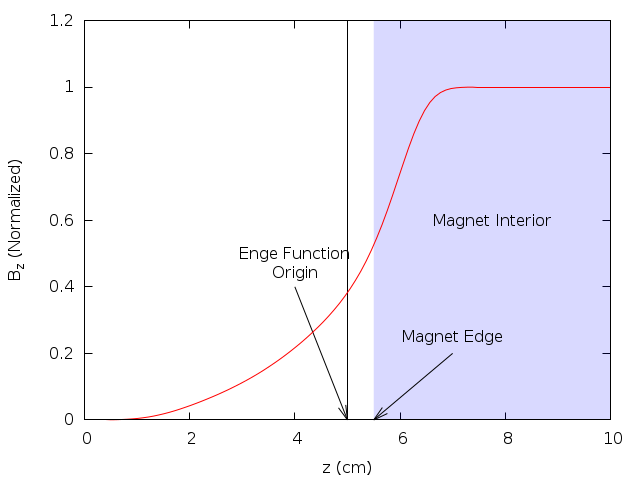
\includegraphics[width=\textwidth]{figures/Elements/Enge-func-plot.png}
\end{center}
\caption{Plot of the entrance fringe field of a dipole magnet along the mid-plane, perpendicular to its entrance face. The field is normalized to 1.0. In this case, the fringe field is described by an Enge function \seeeqn{enge_func} with the parameters from the default \texttt{1DProfile1} field map described in \ssecref{benddefaultfieldmapopalt}. The exit fringe field of this magnet is the mirror image.}
\label{fig:rbend_enge_fringe}
\end{figure}

So far we have described how to setup an \keyword{RBEND} or \keyword{SBEND} element, but have not explained how \opalt uses this information to calculate the magnetic field. The field of both types of magnets is divided into three regions:
\begin{enumerate}
\item Entrance fringe field.
\item Central field.
\item Exit fringe field.
\end{enumerate}
This can be seen clearly in \figref{rbend_field_profile}.

The purpose of the \texttt{1DProfile1} field map \seesec{1DProfile1} associated with the element is to define the Enge functions (\eqnref{enge_func}) that model the entrance and exit fringe fields. To model a particular bend magnet, one must fit the field profile along the mid-plane of the magnet perpendicular to its face for the entrance and exit fringe fields to the Enge function:

\begin{equation}\label{eq:enge_func}
  F(z) = \frac{1}{1 + e^{\sum\limits_{n=0}^{N_{order}} c_{n} (z/D)^{n}}}
\end{equation}
where $D$ is the full gap of the magnet, $N_{order}$ is the Enge function order and $z$ is the distance from the origin
of the Enge function perpendicular to the edge of the dipole. The origin of the Enge function, the order of the Enge function, $N_{order}$, and the constants $c_0$ to $c_{N_{order}}$ are free parameters that are chosen so that the function closely approximates the fringe region of the magnet being modeled. An example of the entrance fringe field is shown in \figref{rbend_enge_fringe}.

Let us assume we have a correctly defined positive \keyword{RBEND} or \keyword{SBEND} element as illustrated in \figref{rbend,sbend}. (As already stated, any bend can be described by a rotated positive bend.) \opalt then has the following information:

\begin{align*}
B_0 &= \text{Field amplitude (T)} \\
R &= \text{Bend radius (m)} \\
n &= -\frac{R}{B_{y}}\diffp{B_y}{x} \text{ (Field index, set using the parameter \keyword{K1})} \\
F(z) &= \left\{
\begin{array}{lll}
	& F_{entrance}(z_{entrance}) \\
	& F_{center}(z_{center}) = 1 \\
	& F_{exit}(z_{exit})
\end{array}
\right.
\end{align*}
Here, we have defined an overall Enge function, $F(z)$, with three parts: entrance, center and exit. The exit and entrance fringe field regions have the form of \eqnref{enge_func} with parameters defined by the \texttt{1DProfile1} field map file given by the element parameter \keyword{FMAPFN}. Defining the coordinates:

\begin{align*}
y &\equiv \text{Vertical distance from magnet mid-plane} \\
\Delta_x &\equiv \text{Perpendicular distance to reference trajectory (see \figref{rbend,sbend})} \\
\Delta_z &\equiv \left\{
\begin{array}{lll}
	& \text{Distance from entrance Enge function origin perpendicular to magnet entrance face.} \\
	& \text{Not defined, Enge function is always 1 in this region.} \\
	& \text{Distance from exit Enge function origin perpendicular to magnet exit face.}
\end{array}
\right.
\end{align*}
using the conditions

\begin{align*}
\nabla \cdot \overrightarrow{B} &= 0 \\
\nabla \times \overrightarrow{B} &= 0
\end{align*}
and making the definitions:

\begin{align*}
F'(z) &\equiv \diff{F(z)}{z} \\
F''(z) &\equiv \diff[2]{F(z)}{z} \\
F'''(z) &\equiv \diff[3]{F(z)}{z}
\end{align*}
we can expand the field off axis, with the result:

\begin{align*}
B_x(\Delta_x, y, \Delta_z) &= -\frac{B_0 \frac{n}{R}}{\sqrt{\frac{n^2}{R^2} +  \frac{F''(\Delta_z)}{F(\Delta_z}}} e^{-\frac{n}{R} \Delta_x} \sin \left[ \left( \sqrt{\frac{n^2}{R^2} + \frac{F''(\Delta_z)}{F(\Delta_z)}} \right) y \right] F(\Delta_z) \\
B_y(\Delta_x, y, \Delta_z) &= B_0 e^{-\frac{n}{R} \Delta_x} \cos \left[ \left( \sqrt{\frac{n^2}{R^2} + \frac{F''(\Delta_z)}{F(\Delta_z)}} \right) y \right] F(\Delta_z) \\
B_z(\Delta_x, y, \Delta_z) &= B_0 e^{-\frac{n}{R} \Delta_x} \left\{\frac{F'(\Delta_z)}{\sqrt{\frac{n^2}{R^2} + \frac{F''(\Delta_z)}{F(\Delta_z)}}} \sin \left[ \left( \sqrt{\frac{n^2}{R^2} + \frac{F''(\Delta_z)}{F(\Delta_z)}} \right) y \right] \right. \\
&- \frac{1}{2 \sqrt{\frac{n^2}{R^2} + \frac{F''(\Delta_z)}{F(\Delta_z)}}} \left(F'''(\Delta_z) - \frac{F'(\Delta_z) F''(\Delta_z)}{F(\Delta_z)} \right) \left[ \frac{\sin \left[ \left( \sqrt{\frac{n^2}{R^2} + \frac{F''(\Delta_z)}{F(\Delta_z)}} \right) y \right]}{\frac{n^2}{R^2} + \frac{F''(\Delta_z)}{F(\Delta_z)}} \right. \\
&- \left. \left. y \frac{\cos \left[ \left( \sqrt{\frac{n^2}{R^2} + \frac{F''(\Delta_z)}{F(\Delta_z)}} \right) y \right]}{\sqrt{\frac{n^2}{R^2} + \frac{F''(\Delta_z)}{F(\Delta_z)}}} \right] \right\}
\end{align*}
These expression are not well suited for numerical calculation, so, we expand them about $y$ to $O(y^2)$ to obtain:

\begin{itemize}
\item In fringe field regions:
\begin{align*}
B_x(\Delta_x, y, \Delta_z) &\approx -B_0 \frac{n}{R} e^{-\frac{n}{R} \Delta_x} y \\
B_y(\Delta_x, y, \Delta_z) &\approx B_0 e^{-\frac{n}{R} \Delta_x} \left[ F(\Delta_z) - \left( \frac{n^2}{R^2} F(\Delta_z) + F''(\Delta_z) \right) \frac{y^2}{2} \right] \\
B_z(\Delta_x, y, \Delta_z) &\approx B_0 e^{-\frac{n}{R} \Delta_x} y F'(\Delta_z)
\end{align*}
\item In central region:
\begin{align*}
B_x(\Delta_x, y, \Delta_z) &\approx -B_0 \frac{n}{R} e^{-\frac{n}{R} \Delta_x} y \\
B_y(\Delta_x, y, \Delta_z) &\approx B_0 e^{-\frac{n}{R} \Delta_x} \left[ 1 -  \frac{n^2}{R^2} \frac{y^2}{2} \right] \\
B_z(\Delta_x, y, \Delta_z) &\approx 0
\end{align*}
\end{itemize}
These are the expressions \opalt uses to calculate the field inside an \keyword{RBEND} or \keyword{SBEND}. First, a particle's position inside the bend is determined (entrance region, center region, or exit region). Depending on the region, \opalt then determines the values of $\Delta_x$, $y$ and $\Delta_z$, and then calculates the field values using the above expressions.

\subsection{Default Field Map (\opalt)}
\label{ssec:benddefaultfieldmapopalt}
\index{RBEND!Default Field Map}
\index{SBEND!Default Field Map}
\index{Default Field Map}
\index{1DPROFILE1-DEFAULT}
Rather than force users to calculate the field of a dipole and then fit that field to find Enge coefficients
for the dipoles in their simulation, we have a default set of values we use from \cite{enge} that are set
when the default field map, ``\keyword{1DPROFILE1-DEFAULT}'' is used:

\begin{align*}
  c_{0} &= 0.478959 \\
  c_{1} &= 1.911289 \\
  c_{2} &= -1.185953 \\
  c_{3} &= 1.630554 \\
  c_{4} &= -1.082657 \\
  c_{5} &= 0.318111
\end{align*}
The same values are used for both the entrance and exit regions of the magnet. In general they will
give good results. (Of course, at some point as a beam line design becomes more advanced, one will want to find
Enge coefficients that fit the actual magnets that will be used in a given design.)

The default field map is the equivalent of the following custom \texttt{1DProfile1} (see \secref{1DProfile1} for an explanation of the field map format) map:

\begin{example}
1DProfile1 5 5 2.0
 -10.0 0.0 10.0 1
 -10.0 0.0 10.0 1
  0.478959
  1.911289
 -1.185953
  1.630554
 -1.082657
  0.318111
  0.478959
  1.911289
 -1.185953
  1.630554
 -1.082657
  0.318111
\end{example}
As one can see, the default magnet gap for ``\keyword{1DPROFILE1-DEFAULT'}'' is set to \SI{2.0}{\centi\meter}. This value
can be overridden by the \keyword{GAP} attribute of the magnet (see \ssecref{RBend,SBend}).

\clearpage

\subsection{SBend3D (OPAL-CYCL)} \label{ssec:SBend3D}
\index{SBEND3D}
% NOTE: SBEND3D, RINGDEFINITION in elements.tex and \ubsection {3D fieldmap} in
% opalcycl.tex all refer to each other - if updating one check for update on
% others to keep them consistent.
The SBend3D element enables definition of a bend from 3D field maps. This can be
used in conjunction with the \keyword{RINGDEFINITION} element to make a ring for
tracking through \opalcycl.

\begin{example}
label: SBEND3D, FMAPFN=string, LENGTH_UNITS=real, FIELD_UNITS=real;
\end{example}

\begin{kdescription}
\item[FMAPFN]
  The field map file name.
\item[LENGTH\_UNITS]
  Units for length (set to 1.0 for units in mm, 10.0 for units in cm, etc).
\item[FIELD\_UNITS]
  Units for field (set to 1.0 for units in T, 0.001 for units in mT, etc).
\end{kdescription}

Field maps are defined using Cartesian coordinates but in a polar geometry with the following restrictions/conventions:
\begin{enumerate}
\item	3D Field maps have to be generated in the vertical direction (z coordinate in \opalcycl) from z = 0 upwards. It cannot be generated symmetrically about z = 0 towards negative z values.
\item	Field map file must be in the form with columns ordered as follows: [$x, z, y, B_{x}, B_{z}, B_{y}$].
\item	Grid points of the position and field strength have to be written on a grid in ($r, z, \theta$) with the primary direction corresponding to the azimuthal direction, secondary to the vertical direction and tertiary to the radial direction.
\end{enumerate}

Below two examples of a \keyword{SBEND3D} which loads a field maps with different units. The \texttt{triplet} example has units of cm and fields units
of Gauss, where the \texttt{Dipole} example (\figref{sbend3d1}) uses meter and Tesla. The first 8 lines in the field map are ignored.

\begin{example}
triplet: SBEND3D, FMAPFN="fdf-tosca-field-map.table", LENGTH_UNITS=10., FIELD_UNITS=-1e-4;
\end{example}

The first few links of the field map \filename{fdf-tosca-field-map.table}:

\begin{example}
      422280      422280      422280           1
 1 X [LENGU]
 2 Y [LENGU]
 3 Z [LENGU]
 4 BX [FLUXU]
 5 BY [FLUXU]
 6 BZ [FLUXU]
 0
 194.01470 0.0000000 80.363520 0.68275932346E-07 -5.3752492577 0.28280706805E-07
 194.36351 0.0000000 79.516210 0.42525693524E-07 -5.3827955117 0.17681348191E-07
 194.70861 0.0000000 78.667380 0.19766168358E-07 -5.4350026348 0.82540823165E-08
.....
\end{example}

\begin{example}
Dipole:SBEND3D,FMAPFN="90degree_Dipole_Magnet.out",LENGTH_UNITS=1000.0, FIELD_UNITS=-10.0;
\end{example}
The first few links of the field map \filename{90degree\_Dipole\_Magnet.out}:
\begin{example}
	4550000	4550000	4550000	1
X [LENGTH_UNITS]
Z [LENGTH_UNITS]
Y [LENGTH_UNITS]
BX [FIELD_UNITS]
BZ [FIELD_UNITS]
BY [FIELD_UNITS]
0
4.3586435e-01   5.0000000e-02   1.2803431e+00   0.0000000e+00   1.6214000e+00   0.0000000e+00
4.2691532e-01   5.0000000e-02   1.2833548e+00   0.0000000e+00   1.6214000e+00   0.0000000e+00
4.1794548e-01   5.0000000e-02   1.2863039e+00   0.0000000e+00   1.6214000e+00   0.0000000e+00
...
\end{example}


This is a restricted feature: \opalcycl.

\begin{figure}[tb]
\begin{center}
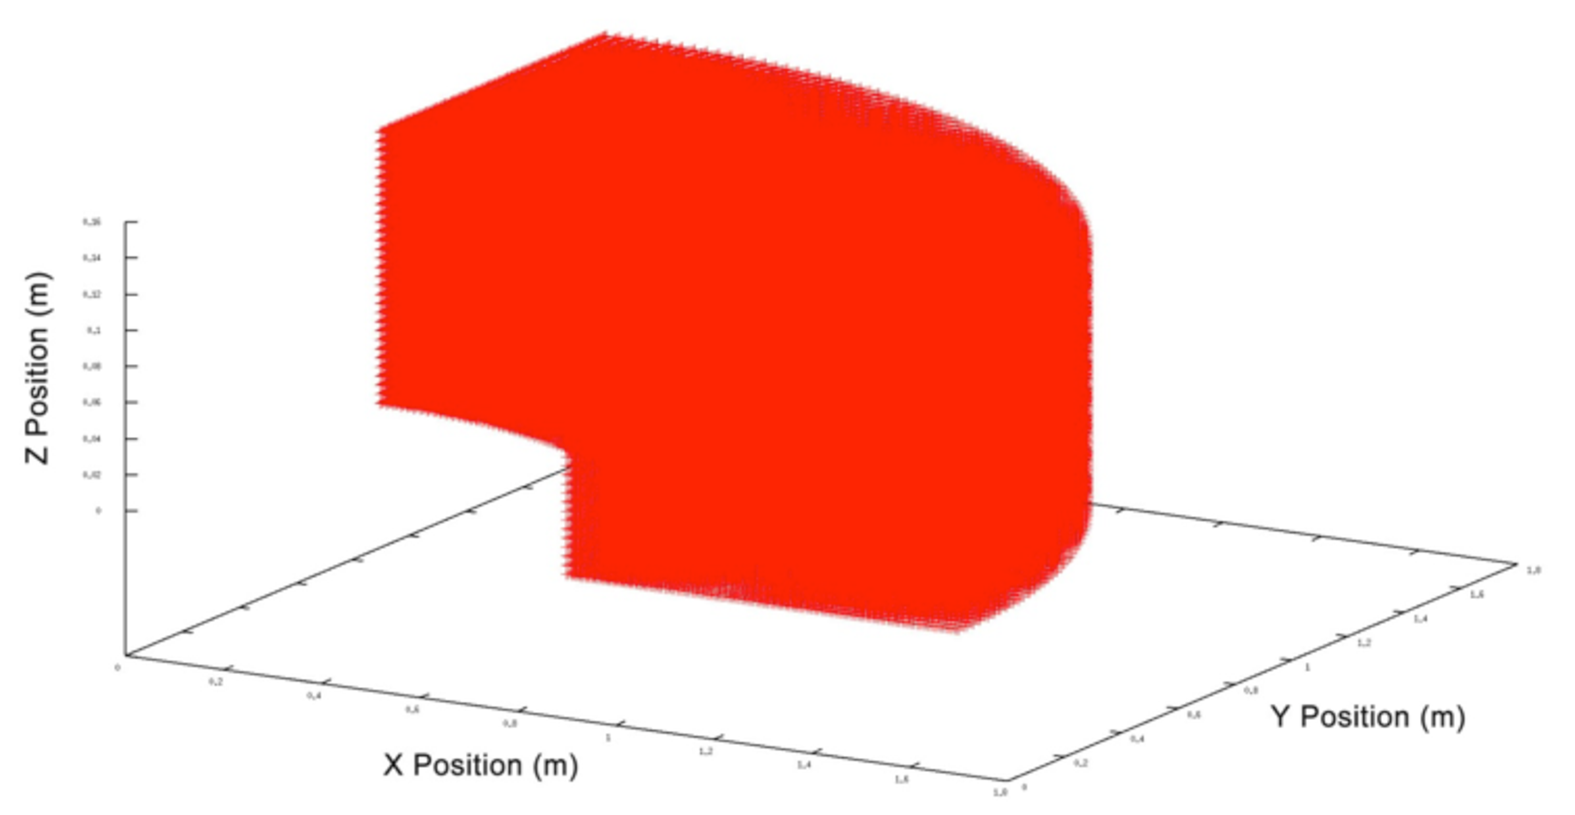
\includegraphics[width=0.58\textwidth]{figures/Elements/sbend3d-1}
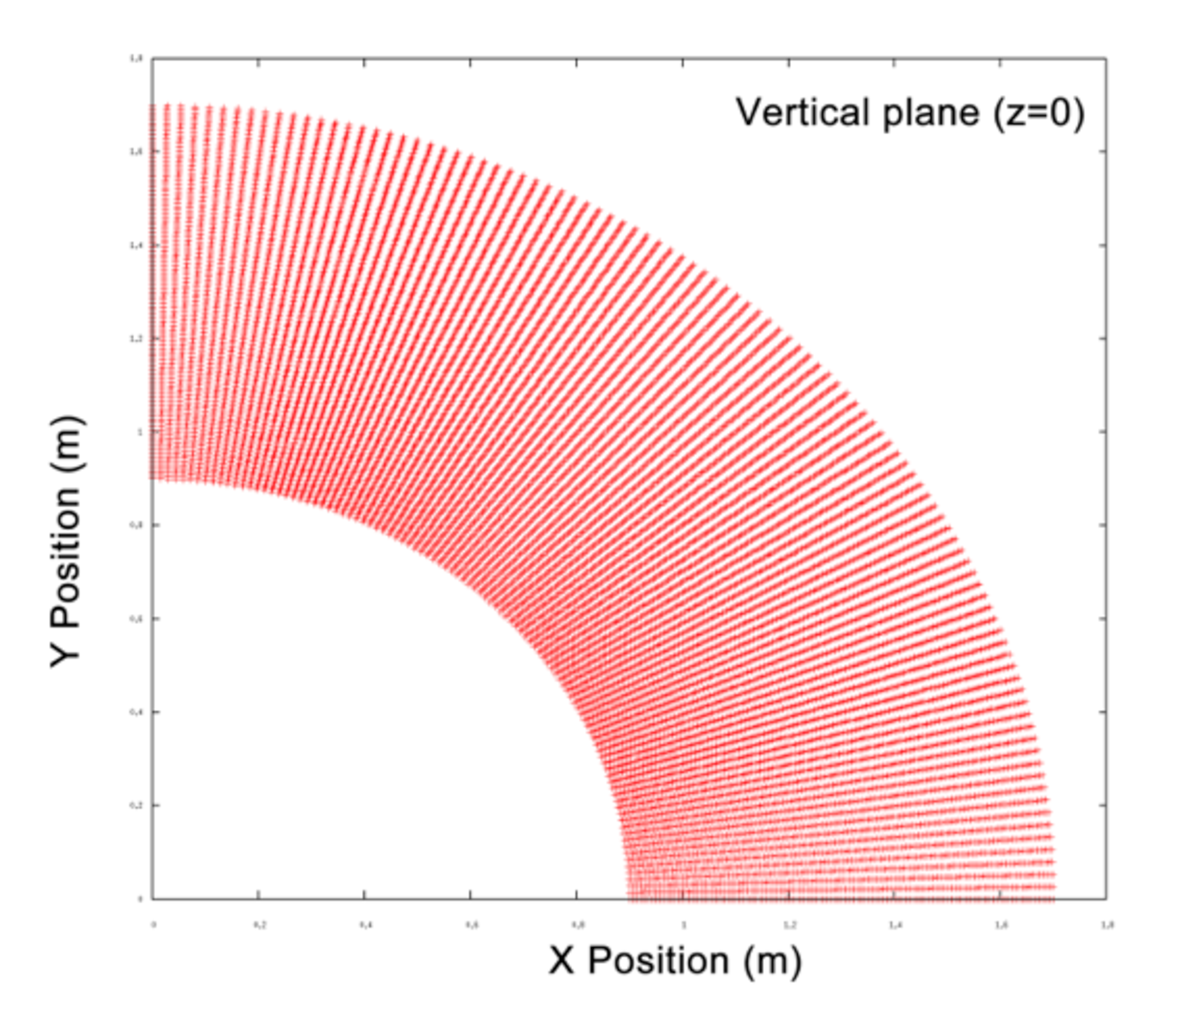
\includegraphics[width=0.4\textwidth]{figures/Elements/sbend3d-2}
\end{center}
\caption{A hard edge model of $90$ degree dipole magnet with homogeneous magnetic field. The right figure
is showing the horizontal cross section of the 3D magnetic field map when $z = 0$}
\label{fig:sbend3d1}
\end{figure}
\index{Bending Magnets|)}



\clearpage
\section{Quadrupole}
\label{sec:quadrupole}
\index{QUADRUPOLE}
\begin{example}
label:QUADRUPOLE, TYPE=string, APERTURE=real-vector,
      L=real, K1=real, K1S=real;
\end{example}

The reference system for a quadrupole is a Cartesian coordinate system
\ifthenelse{\boolean{ShowMap}}{\seefig{straight}}{}. This is a restricted feature:  \noopalcycl.

A \keyword{QUADRUPOLE} has three real attributes:
\begin{kdescription}
\item[K1]
  The normal quadrupole component  $K_1=\diffp{B_y}{x}$.
  The default is $\SI{0}{\tesla\per\meter}$.
  The component is positive, if $B_y$ is positive on the positive $x$-axis.
  This implies horizontal focusing of positively charged particles which
  travel in positive $s$-direction.

\item[K1S]
  The skew quadrupole component. $K_{1s}=-\diffp{B_x}{x}$.
  The default is $\SI{0}{\tesla\per\meter}$.
  The component is negative, if $B_x$ is positive on the positive $x$-axis.
\end{kdescription}

\noindent Example:
\begin{example}
QP1: Quadrupole, L=1.20, ELEMEDGE=-0.5265,
     FMAPFN="1T1.T7", K1=0.11;
\end{example}




\clearpage
\section{Sextupole}
\label{sec:sextupole}
\index{SEXTUPOLE}
\begin{example}
label: SEXTUPOLE, TYPE=string, APERTURE=real-vector,
       L=real, K2=real, K2S=real;
\end{example}
A \keyword{SEXTUPOLE} has three real attributes:
\begin{kdescription}
\item[K2]
  The normal sextupole component
  $K_2=\diffp[2]{B_y}{x}$.
  The default is $\SI{0}{\tesla\per\square\meter}$.
  The component is positive, if $B_y$ is positive on the $x$-axis.
\item[K2S]
  The skew sextupole component
  $K_{2s}=-\diffp[2]{B_x}{x}$.
  The default is $\SI{0}{\tesla\per\square\meter}$.
  The component is negative, if $B_x$ is positive on the $x$-axis.
\end{kdescription}
\noindent Example:
\begin{example}
S:SEXTUPOLE, L=0.4, K2=0.00134;
\end{example}
The reference system for a sextupole is a Cartesian coordinate system
\ifthenelse{\boolean{ShowMap}}{\seefig{straight}}{}.


\clearpage
\section{Octupole}
\label{sec:octupole}
\index{OCTUPOLE}
\begin{example}
label:OCTUPOLE, TYPE=string, APERTURE=real-vector,
      L=real, K3=real, K3S=real;
\end{example}
An \keyword{OCTUPOLE} has three real attributes:
\begin{kdescription}
\item[K3]
  The normal sextupole component
  $K_3=\diffp[3]{B_y}{x}$.
  The default is $\SI{0}{\tesla\meter\tothe{-3}}$.
  The component is positive, if $B_y$ is positive on the positive $x$-axis.
\item[K3S]
  The skew sextupole component
  $K_{3s}=-\diffp[3]{B_x}{x}$.
%  $K_{3s}=\frac{1}{B \rho}\diffp[3]{B_x}{x}$.
  The default is $\SI{0}{\tesla\meter\tothe{-3}}$.
  The component is negative, if $B_x$ is positive on the positive $x$-axis.
\end{kdescription}
\noindent Example:
\begin{example}
O3:OCTUPOLE, L=0.3, K3=0.543;
\end{example}
The reference system for an octupole is a Cartesian coordinate system
\ifthenelse{\boolean{ShowMap}}{\seefig{straight}}{}.

\clearpage
\section{General Multipole}
\label{sec:multipole}
\index{MULTIPOLE}
A \keyword{MULTIPOLE} is in \opalt is of arbitrary order.
\begin{example}
label:MULTIPOLE, TYPE=string, APERTURE=real-vector,
      L=real, KN=real-vector, KS=real-vector;
\end{example}
\begin{kdescription}
\item[KN]
  A real vector \seesec{anarray},
  containing the normal multipole coefficients,
  $K_n=\diffp[n]{B_y}{x}$
  (default is $\SI{0}{\tesla\meter\tothe{-n}}$).
  A component is positive, if $B_y$ is positive on the positive $x$-axis.
\item[KS]
  A real vector \seesec{anarray},
  containing the skew multipole coefficients,
  $K_{n~s}=-\diffp[n]{B_x}{x}$
  (default is $\SI{0}{\tesla\meter\tothe{-n}}$).
  A component is negative, if $B_x$ is positive on the positive $x$-axis.
\end{kdescription}
The order $n$ is unlimited, but all components up to the maximum must be given, even if they are zero.
The number of poles of each component is ($2 n + 2$).

Superposition of many multipole components is permitted.
The reference system for a multipole is a Cartesian coordinate system
\ifthenelse{\boolean{ShowMap}}{\seefig{straight}}{}.

\noindent The following example is equivalent to the quadruple example in \secref{quadrupole}.
\begin{example}
M27:MULTIPOLE, L=1, ELEMEDGE=3.8, KN={0.0,0.11};
\end{example}
A multipole has no effect on the reference orbit, i.e. the reference system at its exit is the same as at its entrance. Use the dipole component only to model a defective multipole.
%If it includes a dipole component,
%it has the same effect on the reference orbit as a \keyword{SBEND}
%with the same length and deflection angle \texttt{KN*L}.

\clearpage
\section{General Multipole (will replace \secref{multipole} when implemented)}
\label{sec:multipoleT}
\index{MULTIPOLET}
A \keyword{MULTIPOLET} is in \opalt a general multipole with extended features. It can represent a straight or curved magnet. In the curved case, the user may choose between constant or variable radius. This model includes fringe fields.  The detailed description can be found at: \url{https://gitlab.psi.ch/OPAL/src/uploads/0d3fc561b57e8962ed79a57cd6115e37/8FBB32A4-7FA1-4084-A4A7-CDDB1F949CD3_psi.ch.pdf}.


\begin{example}
label:MULTIPOLET, L=real, ANGLE=real, VAPERT=real, HAPERT=real,
      LFRINGE=real, RFRINGE=real, TP=real-vector, VARRADIUS=bool;
\end{example}
\begin{kdescription}
\item[L]
  Physical length of the magnet (meters), without end fields. (Default: 1 m)
\item[ANGLE]
  Physical angle of the magnet (radians). If not specified, the magnet is considered to be straight (ANGLE=0.0). This is not the total bending angle since the end fields cause additional bending. The radius of the multipole is set from the LENGTH and ANGLE attributes. 
\item[VAPERT]
  Vertical (non-bend plane) aperture of the magnet (meters). (Default: 0.5 m)
\item[HAPERT]
  Horizontal (bend plane) aperture of the magnet (meters). (Default: 0.5 m)
\item[LFRINGE]
  Length of the left fringe field (meters). (Default: 0.0 m)
\item[RFRINGE]
  Length of the right fringe field (meters). (Default: 0.0 m)
\item[TP]
  A real vector \seesec{anarray}, containing the multipole coefficients of the field expansion on the mid-plane in the body of the magnet: the transverse profile $ T(x) = B_0 + B_1 x + B_2 x^2   + \dots $ is set by TP={$B_0$, $B_1$, $B_2$} (units: $ T \cdot m^{-n}$). The order of highest multipole component is arbitrary, but all components up to the maximum must be given, even if they are zero.
\item[MAXFORDER]
  The order of the maximum function $f_n$ used in the field expansion (default: 5). See the scalar magnetic potential below. This sets for example the maximum power of $z$ in the field expansion of vertical component $B_z$ to $2 \cdot \text{MAXFORDER} $.
\item[EANGLE]
  Entrance edge angle (radians).
\item[ROTATION]
  Rotation of the magnet about its central axis (radians, counterclockwise). This enables to obtain skew fields. (Default 0.0 rad)  
  \item[VARRADIUS]
  This is to be set TRUE if the magnet has variable radius. More precisely, at each point along the magnet, its radius is computed such that the reference trajectory always remains in the centre of the magnet. In the body of the magnet the radius is set from the LENGTH and ANGLE attributes. It is then continuously changed to be proportional to the dipole field on the reference trajectory while entering the end fields. This attribute is only to be set TRUE for a non-zero dipole component. (Default: FALSE) 
\item[VARSTEP]
  The step size (meters) used in calculating the reference trajectory for VARRARDIUS = TRUE. It specifies how often the radius of curvature is re-calculated. This has a considerable effect on tracking time. (Default: 0.1 m)
\end{kdescription}

Superposition of many multipole components is permitted.
The reference system for a multipole is a Cartesian coordinate system for straight
geometry and a $(x,s,z)$ Frenet-Serret coordinate system for curved geometry. In the latter case, the axis $\hat{s}$ is the central axis of the magnet. 






%\clearpage
\clearpage
\section{Solenoid}
\label{sec:solenoid}
\index{SOLENOID}
\begin{example}
label:SOLENOID, TYPE=string, APERTURE=real-vector,
      L=real, KS=real;
\end{example}
A \keyword{SOLENOID} has two real attributes:
\begin{kdescription}
\item[KS]
  The solenoid strength $K_s=\diffp{B_s}{s}$, default is $\SI{0}{\tesla\meter\tothe{-1}}$.
  For positive \keyword{KS} and positive particle charge,
  the solenoid field points in the direction of increasing $s$.
\end{kdescription}
The reference system for a solenoid is a Cartesian coordinate system
\ifthenelse{\boolean{ShowMap}}{\seefig{straight}}{}. Using a solenoid in \opalt mode, the following additional parameters are defined:
\begin{kdescription}
\item[FMAPFN]
  Field maps must be specified.
\end{kdescription}
\noindent Example:
\begin{example}
SP1: Solenoid, L=1.20, ELEMEDGE=-0.5265, KS=0.11,
     FMAPFN="1T1.T7";
\end{example}

\clearpage
\section{Cyclotron}
\label{sec:cyclotron}
\index{CYCLOTRON}
\begin{example}
label:CYCLOTRON, TYPE=string, CYHARMON=int,
      PHIINIT=real, PRINIT=real, RINIT=real,
      SYMMETRY=real, RFFREQ=real, FMAPFN=string;
\end{example}
A \keyword{CYCLOTRON} object includes the main characteristics of a cyclotron, the magnetic field,
 and also the initial condition of the injected reference particle, and it has currently the following attributes:
\begin{kdescription}
\item[TYPE]
    The data format of field map, Currently three formats are implemented:
    CARBONCYCL, CYCIAE, AVFEQ, FFAG, BANDRF and default PSI format.
    For the details of their data format, please read \secref{opalcycl:fieldmap}.
\item[CYHARMON]
    The harmonic number of the cyclotron $h$.
\item[RFFREQ]
    The RF system $f_{rf}$  (unit:MHz, default: 0).
    The particle revolution frequency $f_{rev}$ =  $f_{rf}$ / $h$.
\item[FMAPFN]
    File name for the magnetic field map.
\item[SYMMETRY]
    Defines symmetrical fold number of the B field map data.
\item[RINIT]
    The initial radius of the reference particle (unit: mm, default: 0)
\item[PHIINIT]
    The initial azimuth of the reference particle (unit: degree, default: 0)
\item[ZINIT]
    The initial axial position of the reference particle (unit: mm, default: 0)
\item[PRINIT]
    Initial radial momentum of the reference particle $P_r=\beta_r\gamma$ (default : 0)
\item[PZINIT]
    Initial axial momentum of the reference particle $P_z=\beta_z\gamma$ (default : 0)
\item[MINZ]
    The minimal vertical extent of the machine (unit: mm, default : -10000.0)
\item[MAXZ]
    The maximal vertical extent of the machine (unit: mm, default : 10000.0)
\item[MINR]
    Minimal radial extent of the machine (unit: mm, default : 0.0)
\item[MAXR]
    Minimal radial extent of the machine (unit: mm, default : 10000.0)
\end{kdescription}
During the tracking, the particle ($r, z, \theta$) will be deleted if MINZ $< z <$ MAXZ or MINR $< r <$ MAXR,  and it will be recorded in the ASCII file \filename{\textless inputfilename\textgreater.loss}.
\noindent Example:
\begin{example}
ring: Cyclotron, TYPE="RING", CYHARMON=6, PHIINIT=0.0,
      PRINIT=-0.000240, RINIT=2131.4 , SYMMETRY=8.0,
      RFFREQ=50.650, FMAPFN="s03av.nar",
      MAXZ=10, MINZ=-10, MINR=0, MAXR=2500;
\end{example}

If TYPE is set to BANDRF, the 3D electric field map of RF cavity will be read from external h5part file and 4 extra arguments need to specified:
\begin{kdescription}
\item[RFMAPFN]
The file name for the electric field map in h5part binary format.
\item[RFPHI]
  The Initial phase of the electric field map (rad)
\item[ESCALE]
   The maximal value of the electric field map (MV/m)
\item[SUPERPOSE]
An option whether all of the electric field maps are superposed, The is  valid when more than one electric field map is read. (default: true)
\end{kdescription}
\noindent Example for single electric field map:
\begin{example}
COMET: Cyclotron, TYPE="BANDRF", CYHARMON=2, PHIINIT= -71.0,
PRINIT=pr0, RINIT= r0 , SYMMETRY=1.0, FMAPFN="Tosca_map.txt",
RFPHI=Pi, RFFREQ=72.0,  RFMAPFN="efield.h5part",
ESCALE=1.06E-6;
\end{example}
We can have more than one RF field maps.

\noindent Example for multiple RF field maps:
\begin{example}
COMET: Cyclotron, TYPE="BANDRF", CYHARMON=2, PHIINIT=-71.0,
PRINIT=pr0, RINIT=r0 , SYMMETRY=1.0, FMAPFN="Tosca_map.txt",
RFPHI= {Pi,0,Pi,0}, RFFREQ={72.0,72.0,72.0,72.0},
RFMAPFN={"e1.h5part","e2.h5part","e3.h5part","e4.h5part"},
ESCALE={1.06E-6, 3.96E-6,1.3E-6,1.E-6}, SUPERPOSE=true;
\end{example}
In this example SUPERPOSE is set to true. Therefore, if a particle locates in multiple field regions,  all the field maps are superposed.
if SUPERPOSE is set to  false, then only one field map, which has highest priority,  is used to do interpolation for the particle tracking.
The priority ranking is decided by their sequence in the list of RFMAPFN argument, i.e., "e1.h5hart" has the highest priority and "e4.h5hart" has the lowest priority.

Another method to model an RF cavity is to read the RF voltage profile in the
RFCAVITY element \seesec{cavity} and make a momentum kick when a
particle crosses the RF gap. In the center region of the compact cyclotron, the
electric field shape is complicated and may make a significant impact on
transverse beam dynamics. Hence a simple momentum kick is not enough and we need
to read 3D field map to do precise simulation.

In addition, the simplified trim-coil field model is also implemented so as to
do fine tuning on the magnetic field. A trim-coil can be defined by 4 arguments:
\begin{kdescription}
\item[TCR1]
   Array of inner radii of the trim coils (mm)
\item[TCR2]
   Array of outer radii of the trim coils (mm)
\item[MBTC]
    Array of the maximal B field of the trim coils (kG)
\item[SLPTC]
   Array of the slopes of the rising edge (1/mm)
\end{kdescription}
This is a restricted feature: \opalcycl.

\clearpage
\section{Ring Definition}
\label{sec:ringdefinition}
\index{Ring Definition}
% NOTE: SBEND3D, RINGDEFINITION in elements.tex and \ubsection {3D fieldmap} in
% opalcycl.tex all refer to each other - if updating one check for update on
% others to keep them consistent.

\begin{example}
label: RINGDEFINITION,
       RFFREQ=real, HARMONIC_NUMBER=real, IS_CLOSED=string, SYMMETRY=int,
       LAT_RINIT=real, LAT_PHIINIT=real, LAT_THETAINIT=real,
       BEAM_PHIINIT=real, BEAM_PRINIT=real, BEAM_RINIT=real;
\end{example}

A \keyword{RingDefinition} object contains the main characteristics of a
generalized ring. The \keyword{RingDefinition} lists characteristics of the
entire ring such as harmonic number together with the position of the initial
element and the position of the reference trajectory.

The \keyword{RingDefinition} can be used in combination with \keyword{SBEND3D},
offsets and \keyword{VARIABLE\_RF\_CAVITY} elements to make up a complete ring.

\begin{kdescription}
\item[RFFREQ]
Nominal RF frequency of the ring [\si{\mega\hertz}].

\item[HARMONIC\_NUMBER]
The harmonic number of the ring - i.e. number of bunches in a single pass.

\item[SYMMETRY]
Azimuthal symmetry of the ring. Ring elements will be placed repeatedly
\keyword{SYMMETRY} times.

\item[IS\_CLOSED]
Set to \keyword{FALSE} to disable checking for ring closure.

\item[LAT\_RINIT]
Radius of the first element placement in the lattice [\si{\milli\meter}].

\item[LAT\_PHIINIT]
Azimuthal angle of the first element placed in the lattice [degree].

\item[LAT\_THETAINIT]
Angle in the mid-plane relative to the ring tangent for placement of the first
element [degree].

\item[BEAM\_RINIT]
Initial radius of the reference trajectory [\si{\milli\meter}].

\item[BEAM\_PHIINIT]
Initial azimuthal angle of the reference trajectory [degree].

\item[BEAM\_PRINIT]
Transverse momentum $\beta \gamma$ for the reference trajectory.
\end{kdescription}

In the following example, we define a ring with radius 2.35 m and 4 cells.
\begin{example}
ringdef: RINGDEFINITION, HARMONIC_NUMBER=6, LAT_RINIT=2350.0, LAT_PHIINIT=0.0,
         LAT_THETAINIT=0.0, BEAM_PHIINIT=0.0, BEAM_PRINIT=0.0,
         BEAM_RINIT=2266.0, SYMMETRY=4.0, RFFREQ=0.2;
\end{example}

\subsection{Local Cartesian Offset}
\index{Ring Definition!Local Cartesian Offset}
The \keyword{LOCAL\_CARTESIAN\_OFFSET} enables the user to place an object at an
arbitrary position in the coordinate system of the preceding element. This
enables drift spaces and placement of overlapping elements.
\begin{kdescription}
\item[END\_POSITION\_X] x position of the next element start in the
coordinate system of the preceding element [\si{\milli\meter}].
\item[END\_POSITION\_Y] y position of the next element start in the
coordinate system of the preceding element [\si{\milli\meter}].
\item[END\_NORMAL\_X] x component of the normal vector defining the placement of
the next element in the coordinate system of the preceding element.
\item[END\_NORMAL\_Y] y component of the normal vector defining the placement of
the next element in the coordinate system of the preceding element.
\end{kdescription}

\clearpage
\section{Source}
\label{sec:source}
\index{SOURCE}
This element only works in \opalt. It's only purpose in \opalt is to indicate that the particle source is contained in the beamline. This is needed to place the elements in three-dimensional space when using \keyword{ELEMEDGE}. Otherwise it has no effect on the particles.

\clearpage
\section{RF Cavities (\opalt and \opalcycl)}
\label{sec:cavity}
\index{RFCAVITY}
\index{Cavity}
For an \keyword{RFCAVITY} the three modes have four real attributes in common:
\begin{example}
label:RFCAVITY, APERTURE=real-vector, L=real,
      VOLT=real, LAG=real;
\end{example}
\begin{kdescription}
\item[L]
  The length of the cavity (default: 0~m)
\item[VOLT]
  The peak RF voltage (default: 0~MV).
  The effect of the cavity is
  $\delta E=\text{\keyword{VOLT}}\cdot\sin(2\pi(\text{\keyword{LAG}}-\text{\keyword{HARMON}}\cdot f_0 t))$.
\item[LAG]
  The phase lag [\si{\radian}] (default: 0). In \opalt this phase is in general relative to the phase at which the reference particle gains the most energy. This phase is determined using an auto-phasing algorithm (see~\appref{autophasing}). This auto-phasing algorithm can be switched off, see \keyword{APVETO}.
\end{kdescription}


\subsection{\opalt mode}
\label{sec:cavity-t}
Using a RF Cavity in \opalt mode, the following additional parameters are defined:
\begin{kdescription}
\item[FMAPFN]
  Field maps in the \filename{T7} format can be specified.
\item[TYPE]
  Type specifies STANDING [default] or SINGLE GAP structures.
\item[FREQ]
  Defines the frequency of the RF Cavity in units of MHz. A warning is issued when the frequency of
  the cavity card does not correspond to the frequency defined in the   FMAPFN file. The  frequency of
  the cavity card overrides the  frequency defined in the  FMAPFN file.
\item[APVETO]
  If \keyword{TRUE} this cavity will not be auto-phased. Instead the phase of the cavity is equal to \keyword{LAG} at the arrival time of the reference particle (arrival at the limit of its field {\textbf{not}} at \keyword{ELEMEDGE}).
  \end{kdescription}
\noindent Example standing wave cavity which mimics a DC gun:
\begin{example}
gun: RFCavity, L=0.018, VOLT=-131/(1.052*2.658),
     FMAPFN="1T3.T7", ELEMEDGE=0.00,
     TYPE="STANDING", FREQ=1.0e-6;
\end{example}
\noindent Example of a two frequency standing wave cavity:
\begin{example}
rf1: RFCavity, L=0.54, VOLT=19.961, LAG=193.0/360.0,
     FMAPFN="1T3.T7", ELEMEDGE=0.129, TYPE="STANDING",
     FREQ=1498.956;
rf2: RFCavity, L=0.54, VOLT=6.250, LAG=136.0/360.0,
     FMAPFN="1T4.T7", ELEMEDGE=0.129, TYPE="STANDING",
     FREQ=4497.536;
\end{example}

\subsection{\opalcycl mode}
\label{sec:cavity-cycl}
Using a RF Cavity (standing wave) in \opalcycl mode, the following  parameters are defined:
\begin{kdescription}
\item[FMAPFN]
  Defines name of file which stores normalized voltage amplitude curve of cavity gap in ASCII format.
  (See data format in \secref{opalcycl:rffieldmap})
 \item[VOLT]
  Sets peak value of voltage amplitude curve in MV.
  \item[TYPE]
  Defines Cavity type, SINGLEGAP represents cyclotron type cavity.
  \item[FREQ]
  Sets the frequency of the RF Cavity in units of MHz.
  \item[RMIN]
  Sets the radius of the cavity inner edge in mm.
  \item[RMAX]
  Sets the radius of the cavity outer edge in mm.

  \item[ANGLE]
  Sets the azimuthal position of the cavity in global frame in degree.

  \item[PDIS]
  Set shift distance of cavity gap from center of cyclotron in mm. If its value is positive,
  the shift direction is clockwise, namely, shift towards the smaller azimuthal angle.

  \item[GAPWIDTH]
  Set gap width of  cavity in mm.

  \item[PHI0]
  Set initial phase of cavity in degree.

\end{kdescription}

\noindent Example of a RF cavity of cyclotron:
\begin{example}
rf0: RFCavity, VOLT=0.25796, FMAPFN="Cav1.dat",
     TYPE="SINGLEGAP", FREQ=50.637, RMIN = 350.0,
     RMAX = 3350.0, ANGLE=35.0,   PDIS = 0.0,
     GAPWIDTH = 0.0, PHI0=phi01;
\end{example}

\figref{Cyclotron_cavity} shows the simplified geometry of a cavity gap and its parameters.

\begin{figure}[hbt]
  \centering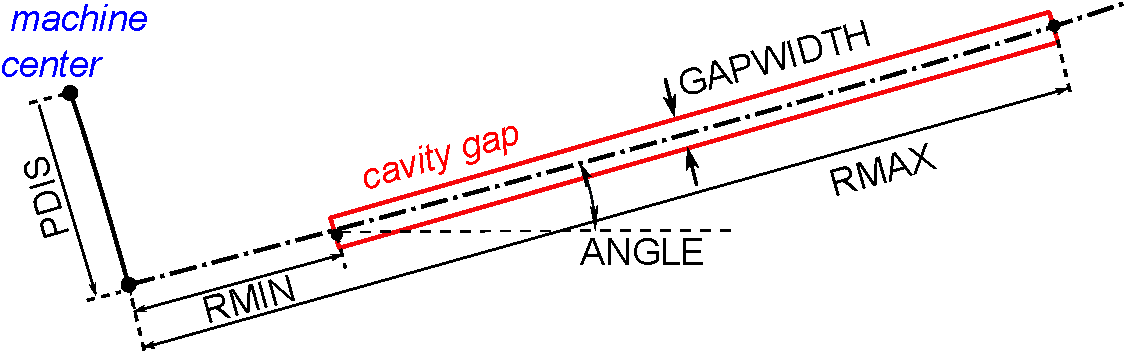
\includegraphics[scale=0.6]{./figures/cyclotron/Cavity.pdf}
  \caption{Schematic of the simplified geometry of a cavity gap and parameters}
  \label{fig:Cyclotron_cavity}
\end{figure}

\clearpage
\section{RF Cavities with Time Dependent Parameters}
\label{sec:variable-rf-cavity-cycl}
\index{RFCavity!Variable}
\index{Cavity!Variable}
The \keyword{VARIABLE\_RF\_CAVITY} element can be used to define RF Cavities with
Time Dependent Parameters in \opalcycl mode. Variable RF Cavities must be
placed using the \keyword{RingDefinition} element.
\begin{kdescription}
\item[FREQUENCY\_MODEL]
  String naming the time dependence model of the cavity frequency, $f$ [\si{\mega\hertz}].
\item[AMPLITUDE\_MODEL]
  String naming the time dependence model of the cavity amplitude, $E_0$ [\si{\mega\volt/\meter}].
\item[PHASE\_MODEL]
  String naming the time dependence model of the cavity phase offset, $\phi$.
\item[WIDTH]
  Full width of the cavity [\si{\milli\meter}].
  \item[HEIGHT]
  Full height of the cavity [\si{\milli\meter}].
  \item[L]
  Full length of the cavity [\si{\milli\meter}].
\end{kdescription}
The field inside the cavity is given by
\begin{equation}
\vec{E} = \big(0, 0, E_0(t)\sin[2\pi f(t) t+\phi(t)]\big)
\end{equation}
with no field outside the cavity boundary. There is no magnetic field or
transverse dependence on electric field.

\subsection{Time Dependence}
\label{sec:polynomial-time-dependence}
\index{RFCavity!Time Dependence}
\index{Cavity!Time Dependence}
The \keyword{POLYNOMIAL\_TIME\_DEPENDENCE} element is used to define time dependent
parameters in RF cavities in terms of a \engordnumber{4} order polynomial.
\begin{kdescription}
\item[P0]
  Constant term in the polynomial expansion.
\item[P1]
  First order term in the polynomial expansion [ns$^{-1}$].
\item[P2]
  Second order term in the polynomial expansion [ns$^{-2}$].
  \item[P3]
  Third order term in the polynomial expansion [ns$^{-3}$].
  %% \item[P4]
  %% Fourth order term in the polynomial expansion [ns$^{-4}$].
\end{kdescription}
The polynomial is evaluated as
\begin{equation}
g(t) = p_0 + p_1 t + p_2 t^2 + p_3 t^3 %% + p_4 t^4
.
\end{equation}

An example of a Variable Frequency RF cavity of cyclotron with polynomial
time dependence of parameters is given below:
\begin{example}
REAL phi=2.*PI*0.25;

REAL rf_p0=0.00158279;
REAL rf_p1=9.02542e-10;
REAL rf_p2=-1.96663e-16;
REAL rf_p3=2.45909e-23;

RF_FREQUENCY: POLYNOMIAL_TIME_DEPENDENCE, P0=rf_p0, P1=rf_p1, P2=rf_p2, P3=rf_p3;
RF_AMPLITUDE: POLYNOMIAL_TIME_DEPENDENCE, P0=1.0;
RF_PHASE: POLYNOMIAL_TIME_DEPENDENCE, P0=phi;

RF_CAVITY: VARIABLE_RF_CAVITY, PHASE_MODEL="RF_PHASE", AMPLITUDE_MODEL="RF_AMPLITUDE",
           FREQUENCY_MODEL="RF_FREQUENCY", L=100., HEIGHT=200., WIDTH=2000.;
\end{example}

\clearpage
\section{Traveling Wave Structure}
\label{sec:travelingwave}
\index{TRAVELINGWAVE}

%======================FIGURE===============================
\begin{figure}[tb]
\centering
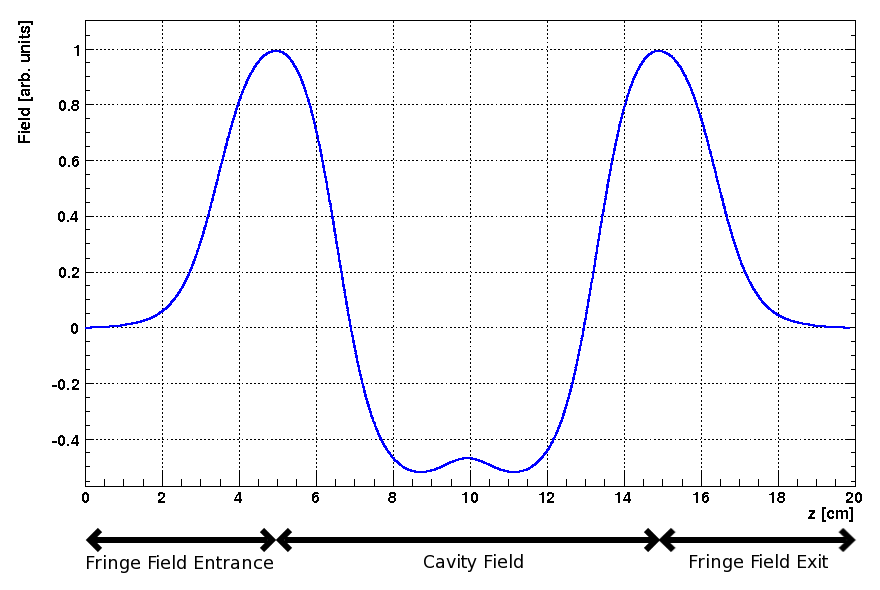
\includegraphics[width=0.7\textwidth]{./figures/traveling-wave-structure/FINSB-RAC-field.png}
\caption[The on-axis field of an S-band \keyword{TRAVELINGWAVE} structure]{The on-axis field of an S-band (2997.924~MHz) \keyword{TRAVELINGWAVE} structure.
    The field of a single cavity is shown between its entrance and exit fringe fields.
    The fringe fields extend one half wavelength ($\lambda/2$) to either side.}
\label{fig:FINSB-RAC-field}
\end{figure}
%===========================================================

\begin{figure}[hbt]
  \centering
\end{figure}

An example of a 1D \keyword{TRAVELINGWAVE} structure field map is shown in \figref{FINSB-RAC-field}.
This map is a standing wave solution generated by Superfish and shows the field on axis for a single accelerating cavity with
the fringe fields of the structure extending to either side. \opalt reads in this field map and constructs the total field of the
\keyword{TRAVELINGWAVE} structure in three parts: the entrance fringe field, the structure fields and the exit fringe field.

The fringe fields are treated as standing wave structures and are given by:
\begin{equation*}
  \begin{aligned}
    \vec{E_{entrance}}(\vec{r}, t) &= \vec{E_{from-map}}(\vec{r}) \cdot \text{\keyword{VOLT}} \cdot \cos \left( 2\pi \cdot \text{\keyword{FREQ}} \cdot t
        + \phi_{entrance} \right) \\
    \vec{E_{exit}}(\vec{r}, t) &= \vec{E_{from-map}}(\vec{r}) \cdot \text{\keyword{VOLT}} \cdot \cos \left( 2\pi \cdot \text{\keyword{FREQ}} \cdot t
        + \phi_{exit} \right)
  \end{aligned}
\end{equation*}
where VOLT and FREQ are the field magnitude and frequency attributes (see below).
$ \phi_{entrance}= \text{\keyword{LAG}}$, the phase attribute of the element (see below). $ \phi_{exit} $ is dependent upon both LAG and the NUMCELLS
attribute (see below) and is calculated internally by \opalt.

The field of the main accelerating structure is reconstructed from the center section of the standing wave solution shown in
\figref{FINSB-RAC-field} using

\begin{equation*}
  \begin{split}
    \vec{E} ( \vec{r},t ) &= \frac{\text{\keyword{VOLT}}}{\sin (2 \pi \cdot \text{\keyword{MODE}})} \\
    &\phantom{=}
    \times \Biggl\{ \vec{E_{from-map}} (x,y,z) \cdot \cos \biggl( 2 \pi \cdot \text{\keyword{FREQ}} \cdot t + \text{\keyword{LAG}}+ \frac{\pi}{2} \cdot \text{\keyword{MODE}} \Bigr) \\
    &\phantom{= \times \Biggl\{}
    + \vec{E_{from-map}}(x,y,z+d) \cdot \cos \biggl( 2 \pi \cdot \text{\keyword{FREQ}} \cdot t + \text{\keyword{LAG}} + \frac{3 \pi}{2} \cdot \text{\keyword{MODE}} \Bigr) \Biggr\}
  \end{split}
\end{equation*}
where d is the cell length and is defined as $\text{d} = \lambda \cdot \text{\keyword{MODE}} $. MODE is an attribute of the element (see below).
When calculating the field from the map ($\vec{E_{from-map}}(x,y,z)$), the longitudinal position is referenced to the start of the cavity fields
at $\frac{\lambda}{2}$ (In this case starting at $z = \SI{5.0}{\centi\meter}$). If the longitudinal position advances past the end of the cavity map
($\frac{3\lambda}{2} = \SI{15.0}{\centi\meter}$ in this example), an integer number of cavity wavelengths is subtracted from the position until it is back
within the map's longitudinal range.

A \keyword{TRAVELINGWAVE} structure has seven real attributes, one integer attribute, one string attribute and one Boolean attribute:
\begin{example}
label:TRAVELINGWAVE, APERTURE=real-vector, L=real,
      VOLT=real, LAG=real, FMAPFN=string,
      ELEMEDGE=real, FREQ=real, NUMCELLS=integer,
      MODE=real;
\end{example}

\begin{kdescription}
\item[L]
  The length of the cavity (default: 0~m). In \opalt this attribute is ignored, the length is defined by the field map and the number of cells.
\item[VOLT]
  The peak RF voltage (default: 0~MV).
  The effect of the cavity is
  $\delta E=\text{\keyword{VOLT}}\cdot\sin(\text{\keyword{LAG}}- 2\pi\cdot\text{\keyword{FREQ}}\cdot t)$.
\item[LAG]
  The phase lag [\si{\radian}] (default: 0). In \opalt this phase is in general relative to the phase at which the reference particle gains the most energy. This phase is determined using an auto-phasing algorithm (see~\appref{autophasing}). This auto-phasing algorithm can be switched off, see \keyword{APVETO}.
\item[FMAPFN]
  Field maps in the \filename{T7} format can be specified.
\item[FREQ]
  Defines the frequency of the traveling wave structure in units of MHz. A warning is issued when the frequency of
  the cavity card does not correspond to the frequency defined in the  FMAPFN file. The frequency defined in the FMAPFN
  file overrides the frequency defined on the cavity card.
\item[NUMCELLS]
  Defines the number of cells in the tank. (The cell count should not include the entry and exit half cell fringe fields.)
\item[MODE]
Defines the mode in units of $2\pi$, for example $\frac{1}{3}$ stands for a $\frac{2 \pi}{3}$ structure.
\item[FAST]
If FAST is true and the provided field map is in 1D then a 2D field map is constructed from the 1D on-axis field, see \secref{fieldmaps}. To track the particles the field values are interpolated from this map instead of using an FFT based algorithm for each particle and each step. (default: FALSE)
\item[APVETO]
  If \keyword{TRUE} this cavity will not be auto-phased. Instead the phase of the cavity is equal to \keyword{LAG} at the arrival time of the reference particle (arrival at the limit of its field {\textbf{not}} at \keyword{ELEMEDGE}).
\end{kdescription}

\noindent Use of a traveling wave requires the particle momentum \texttt{P}
and the particle charge \keyword{CHARGE} to be set on the relevant
optics command before any calculations are performed.

Example of a L-Band traveling wave structure:
\begin{example}
lrf0: TravelingWave, L=0.0253, VOLT=14.750,
      NUMCELLS=40, ELEMEDGE=2.73066,
      FMAPFN="INLB-02-RAC.Ez", MODE=1/3,
      FREQ=1498.956, LAG=248.0/360.0;
\end{example}




\clearpage
\section{Monitor}
\label{sec:monitor}
\index{MONITOR}
 A \keyword{MONITOR} detects all particles passing it and writes the position, the momentum and the time when they hit it into an H5hut file. Furthermore the exact position of the monitor is stored. It has always a length of \SI{1}{\centi\meter} consisting of \SI{0.5}{\centi\meter} drift, the monitor of zero length and another \SI{0.5}{\centi\meter} drift. This is to prevent \opalt from missing any particle. The positions of the particles on the monitor are interpolated from the current position and momentum one step before they would passe the monitor.
\begin{kdescription}
\item[OUTFN]
  The file name into which the monitor should write the collected data. The file is an H5hut file.
\end{kdescription}

If the attribute \keyword[sec:Element:common]{TYPE} is set to \keyword{TEMPORAL} then the data of all particles are written to the H5hut file when the reference particle hits the monitor.

This is a restricted feature:  \noopalcycl.

%\section{Gun}
%\label{sec:gun}
%\index{gun}
%The gun uses the defined distribution \seechp{distribution} and emits particles for a given duration (eventually defined
%by the laser duration).  The temperature is defined by the parameters on the distribution command.

%\begin{example}
%g1:GUN, TYPE=string, TEMISSION=real, L=real, EMISSIONSLICES=real;
%\end{example}
%The gun has beside the standard attribute TYPE,  four more attributes:
%\begin{kdescription}
%\item[L]
%  The gun length (default: 0~m).
%\item[TEMISSION]
%  The time-span  at which emission occurs (default: 0~sec).
%\item[EMISSIONSLICES]
%  How many emission slices we consider (default: 0).
%\end{kdescription}

%\noindent Example:
%\begin{example}
%G1:GUN, L=6.0E-3, TEMISSION= 36E-12, EMISSIONSLICES=360;
%\end{example}
%The reference system for a gun is a Cartesian coordinate system
%\ifthenelse{\boolean{ShowMap}}{ \seeref{straight}}{}.


\clearpage
\section{Collimators}
\label{sec:collimators}
\index{Collimators|(}
Three types of collimators are defined:
\begin{kdescription}
\item[ECOLLIMATOR]
  \label{sec:ecollimator}
  Elliptic aperture,
\item[RCOLLIMATOR]
  \label{sec:rcollimator}
  Rectangular aperture.
\item[CCOLLIMATOR]
  \index{CCOLLIMATOR}
   Radial rectangular collimator in cyclotrons

\end{kdescription}
\begin{example}
label:ECOLLIMATOR, TYPE=string, APERTURE=real-vector,
      L=real, XSIZE=real, YSIZE=real;
label:RCOLLIMATOR,TYPE=string, APERTURE=real-vector,
      L=real, XSIZE=real, YSIZE=real;
\end{example}
Either type has three real attributes:
\begin{kdescription}
\item[L]
  The collimator length (default: 0~m).
\item[XSIZE]
  The horizontal half-aperture (default: unlimited).
\item[YSIZE]
  The vertical half-aperture (default: unlimited).
\end{kdescription}
For elliptic apertures,
\keyword{XSIZE} and \keyword{YSIZE} denote the half-axes respectively,
for rectangular apertures they denote the half-width of the rectangle.
Optically a collimator behaves like a drift space, but during tracking,
it also introduces an aperture limit.
The aperture is checked at the entrance.
If the length is not zero, the aperture is also checked at the exit.

\noindent Example:
\begin{example}
COLLIM:ECOLLIMATOR, L=0.5, XSIZE=0.01, YSIZE=0.005;
\end{example}
The reference system for a collimator is a Cartesian coordinate system
\ifthenelse{\boolean{ShowMap}}{\seefig{straight}}{}.


\subsection{\opalt mode}
 The \keyword{CCOLLIMATOR} isn't supported. \keyword{ECOLLIMATOR}s and \keyword{RCOLLIMATOR}s detect all particles which are outside the aperture defined by
\keyword{XSIZE} and \keyword{YSIZE}. Lost particles are saved in an H5hut file defined by \keyword{OUTFN}. The \keyword{ELEMEDGE} defines the location of the collimator and \keyword{L} the length.
\begin{kdescription}
\item[OUTFN]
  The file name into which the monitor should write the collected data. The file is an H5hut file.
\end{kdescription}

\noindent Example:
\begin{example}
Col:ECOLLIMATOR, L=1.0E-3, ELEMEDGE=3.0E-3, XSIZE=5.0E-4,
    YSIZE=5.0E-4, OUTFN="Coll.h5";
\end{example}


\subsection{\opalcycl mode}

Only \keyword{CCOLLIMATOR} is available for \opalcycl.  This element is radial rectangular collimator which can be used to collimate the radial tail particles.
So when a particle hit this collimator, it will be absorbed or scattered, the algorithm is based on the Monte Carlo method .
Pleased note when a particle is scattered, it will not be recorded as the lost particle.
If this particle leave the bunch, it will be removed during the integration afterwards, so as to maintain the accuracy of space charge solving.

\begin{kdescription}
\item[XSTART]
The x coordinate of the start point. [\si{\milli\meter}]
 \item[XEND]
The x coordinate of the end point. [\si{\milli\meter}]
\item[YSTART]
The y coordinate of the start point. [\si{\milli\meter}]
 \item[YEND]
The y coordinate of the end point. [\si{\milli\meter}]
\item[ZSTART]
The vertical coordinate of the start point [\si{\milli\meter}]. Default value is \SI{-100}{\milli\meter}.
 \item[ZEND]
The vertical coordinate of the end point. [\si{\milli\meter}]. Default value is \SI{-100}{\milli\meter}.
\item[WIDTH]
The width of the septum. [\si{\milli\meter}]
 \item[PARTICLEMATTERINTERACTION]
\keyword{PARTICLEMATTERINTERACTION} is an attribute of the element. Collimator physics is only a kind of particlematterinteraction.
 It can be applied to any element. If the type of \keyword{PARTICLEMATTERINTERACTION} is \keyword{COLLIMATOR}, the material is defined here.
 The material ``Cu", ``Be", ``Graphite" and ``Mo" are defined until now.
 If this is not set, the particle matter interaction module will not be activated.
 The particle hitting collimator will be recorded and directly deleted from the simulation.
\end{kdescription}

\begin{tikzpicture}[scale=1.5,axis/.style={very thick, ->, >=stealth'}]
    % Draw axes
    \draw [->,thick] (1,-2.0) -- (1,2.0) node (yaxis) [above] {$y$};
    \draw [->,thick] (-1.2,1.0)  -- (4.0,1.0) node (xaxis) [right] {$x$};
    \draw (3.5,-0.2) --(2.0,-1.5)
          (2.0,-1.5) --(2.5,-2.0)
          (2.5,-2.0) --(4.0,-0.7)
          (4.0,-0.7) --(3.5,-0.2);
    \fill[red] (2.25,-1.75)  circle (1pt) node (start)[below] {(xstart,ystart)};
    \fill[red] (3.75,-0.45)  circle (1pt) node (end)[above] {(xend,yend)};
    \node (collimator) at (2.55,-0.55)[anchor=mid] {collimator};
    \draw [<->,thick,blue] (2.75,-0.85)--(3.25,-1.35) node [right] {width};

\end{tikzpicture}


\noindent Example:
\begin{example}
REAL y1=-0.0;
REAL y2=0.0;
REAL y3=200.0;
REAL y4=205.0;
REAL x1=-215.0;
REAL x2=-220.0;
REAL x3=0.0;
REAL x4=0.0;
cmphys:particlematterinteraction, TYPE="Collimator", MATERIAL="Cu";
cma1: CCollimator, XSTART=x1, XEND=x2,YSTART=y1, YEND=y2,
ZSTART=2, ZEND=100, WIDTH=10.0, PARTICLEMATTERINTERACTION=cmphys ;
cma2: CCollimator, XSTART=x3, XEND=x4,YSTART=y3, YEND=y4,
 ZSTART=2, ZEND=100, WIDTH=10.0, PARTICLEMATTERINTERACTION=cmphys;
\end{example}

The particles lost on the CCOLLIMATOR are recorded in the ASCII file \filename{\textless inputfilename\textgreater.loss}
\index{Collimators|)}

\clearpage
\section{Septum (\opalcycl)}
\index{SEPTUM}
This is a restricted feature: \noopalt.
The particles hitting on the septum is removed from the bunch. There are 5 parameters to describe a septum.
\begin{kdescription}
\item[XSTART]
The x coordinate of the start point. [\si{\milli\meter}]
 \item[XEND]
The x coordinate of the end point. [\si{\milli\meter}]
\item[YSTART]
The y coordinate of the start point. [\si{\milli\meter}]
 \item[YEND]
The y coordinate of the end point. [\si{\milli\meter}]
\item[WIDTH]
The width of the septum. [\si{\milli\meter}]
\end{kdescription}

\begin{tikzpicture}[scale=1.5,axis/.style={very thick, ->, >=stealth'}]
    % Draw axes
    \draw [->,thick] (1,-2.0) -- (1,2.0) node (yaxis) [above] {$y$};
    \draw [->,thick] (-1.2,1.0)  -- (4.0,1.0) node (xaxis) [right] {$x$};
    \draw (3.5,-0.2) --(2.0,-1.5)
          (2.0,-1.5) --(2.1,-1.6)
          (2.1,-1.6) --(3.6,-0.3)
          (3.6,-0.3) --(3.5,-0.2);
    \fill[red] (2.05,-1.55)  circle (1pt) node (start)[below] {(xstart,ystart)};
    \fill[red] (3.55,-0.25)  circle (1pt) node (end)[above] {(xend,yend)};
    \node (steptum) at (2.55,-0.55)[anchor=mid] {septum};
    \draw [<->,thick,blue] (2.75,-0.85)--(2.85,-0.95) node [right] {width};

\end{tikzpicture}

\noindent Example:
\begin{example}
eec2: Septum, xstart=4100.0, xend=4300.0,
ystart=-1200.0, yend=-150.0, width=0.05;
\end{example}

The particles lost on the SEPTUM are recorded in the ASCII file \filename{\textless input\_file\_name \textgreater.loss}.

\clearpage
\section{Probe (\opalcycl)}
\index{PROBE}
The particles hitting on the probe is recorded. There are 5 parameters to describe a probe.
\begin{kdescription}
\item[XSTART]
The x coordinate of the start point. [\si{\milli\meter}]
 \item[XEND]
The x coordinate of the end point. [\si{\milli\meter}]
\item[YSTART]
The y coordinate of the start point. [\si{\milli\meter}]
 \item[YEND]
The y coordinate of the end point. [\si{\milli\meter}]
\item[WIDTH]
 The width of the probe, NOT used yet.
\end{kdescription}

\begin{tikzpicture}[scale=1.5,axis/.style={very thick, ->, >=stealth'}]
    % Draw axes
    \draw [->,thick] (0.5,-2.0) -- (0.5,2.0) node (yaxis) [above] {$y$};
    \draw [->,thick] (-1.2,1.0)  -- (4.0,1.0) node (xaxis) [right] {$x$};
    \draw (1.5,-0.5) --(3.0,-1.5)
          (3.0,-1.5) --(3.1,-1.4)
          (3.1,-1.4) --(1.6,-0.4)
          (1.6,-0.4) --(1.5,-0.5);
    \fill[red] (1.55,-0.45)  circle (1pt) node (start)[above] {(xstart,ystart)};
    \fill[red] (3.05,-1.45)  circle (1pt) node (end)[below] {(xend,yend)};
    \node (steptum) at (2.55,-0.55)[anchor=mid] {probe};
    \draw [<->,thick,blue] (2.25,-1.0)--(2.35,-0.9) node [right] {width};
\end{tikzpicture}

\noindent Example:
\begin{example}
prob1: Probe, xstart=4166.16, xend=4250.0,
ystart=-1226.85, yend=-1241.3;
\end{example}
The particles probed on the PROBE are recorded in the ASCII file \filename{\textless inputfilename\textgreater.loss}.
Please note that  these particles are not deleted in the simulation, however, they are recorded in the ``loss" file.


\clearpage
\section{Stripper (\opalcycl)}
\index{STRIPPER}
A stripper element strip the electron(s) from a particle. The particle hitting the stripper is recorded in the file,
which contains the time, coordinates and momentum of the particle at the moment it hit the stripper.
The charge and mass are changed. Its has the same geometry as the PROBE element.
Please note that the stripping physics in not included yet.

 There are 9 parameters to describe a stripper.
\begin{kdescription}
\item[XSTART]
The x coordinate of the start point. [\si{\milli\meter}]
 \item[XEND]
The x coordinate of the end point. [\si{\milli\meter}]
\item[YSTART]
The y coordinate of the start point. [\si{\milli\meter}]
 \item[YEND]
The y coordinate of the end point. [\si{\milli\meter}]
\item[WIDTH]
 The width of the probe, NOT used yet.
\item[OPCHARGE]
Charge number of the out-coming particle. Negative  value represents negative charge.
\item[OPMASS]
Mass of the out-coming particles. [\si{\giga\electronvolt/\clight\squared}]
\item[OPYIELD]
Yield of the out-coming particle (the outcome particle number per income particle) , the default value is 1.
\item[STOP]
If STOP is true, the particle is stopped and deleted from the simulation;
Otherwise, the out-coming particle continues to be tracked along the extraction path.
\end{kdescription}

\noindent Example: $H_2^+$ particle stripping
\begin{example}
prob1: Stripper, xstart=4166.16, xend=4250.0,
ystart=-1226.85, yend=-1241.3,
opcharge=1, opmass=PMASS, opyield=2, stop=false;
\end{example}

No matter what the value of STOP is, the particles hitting on the STRIPPER are recorded in the ASCII file \filename{\textless inputfilename\textgreater.loss}.



\clearpage
\section{Degrader (\opalt)}
\index{DEGRADER}
Elliptical degrader with an overall length \keyword{L}.
\begin{kdescription}
\item[XSIZE]
\index[XSIZE]
Major axis of the transverse elliptical shape, default value is 1e6.
\item[YSIZE]
Minor axis of the transverse elliptical shape, default value is 1e6.
\end{kdescription}
\noindent Example: Graphite degrader of \SI{15}{\centi\meter} thickness.
\begin{example}
DEGPHYS: PARTICLEMATTERINTERACTION, TYPE="DEGRADER", MATERIAL="Graphite";

DEG1: DEGRADER, L=0.15, ELEMEDGE=0.02, PARTICLEMATTERINTERACTION=DEGPHYS;
\end{example}



\clearpage
\section{Correctors (\opalt)}
\label{sec:corrector}
\index{Correctors}
Three types of correctors are available:
\begin{kdescription}
\item[HKICKER]
  \label{sec:hkicker}
  A corrector for the horizontal plane.
\item[VKICKER]
  \label{sec:vkicker}
  A corrector for the vertical plane.
\item[KICKER]
  \label{sec:kicker}
  A corrector for both planes.
\end{kdescription}
They act as
\begin{example}
label:HKICKER, TYPE=string, APERTURE=real-vector,
      L=real, KICK=real;
label:VKICKER, TYPE=string, APERTURE=real-vector,
      L=real, KICK=real;
label:KICKER, TYPE=string, APERTURE=real-vector,
      L=real, HKICK=real, VKICK=real;
\end{example}
They have the following attributes:
\begin{kdescription}
\item[L]
  The length of the closed orbit corrector (default: 0~m).
\item[KICK]
  The kick angle in \si{\radian} for either horizontal or vertical correctors
  (default: \SI{0}{\radian}).
\item[HKICK]
  The horizontal kick angle in \si{\radian} for a corrector in both planes
  (default: \SI{0}{\radian}).
\item[VKICK]
  The vertical kick angle in \si{\radian} for a corrector in both planes
  (default: \SI{0}{\radian}).
\item[DESIGNENERGY]
  Fix the magnitude of the magnetic field using the given \keyword{DESIGNENERGY} and the angle (\keyword{KICK}, \keyword{HKICK} or \keyword{VKICK}). If the designenergy isn't set then the actual energy of the reference particle at the position of the corrector is used. The \keyword{DESIGNENERGY} is expected in \si{\mega\electronvolt}.
\end{kdescription}
A positive kick increases $p_{x}$ or $p_{y}$
respectively. Use \keyword{KICK} for an \keyword{HKICKER} or \keyword{VKICKER} and \keyword{HKICK} and \keyword{VKICK} for a \keyword{KICKER}. Instead of using a \keyword{KICKER} or a \keyword{VKICKER} one could use an \keyword{HKICKER} and rotate it appropriately using \keyword[sec:Element:common]{PSI}.

Correctors don't change the reference trajectory. Otherwise they are implemented as \keyword{RBEND} with $\texttt{E1} = 0$ and without fringe fields (hard edge model). They can be used to model earth's magnetic field which is neglected in the design trajectory but which has a noticeable effect on the trajectory of a bunch at low energies.

\noindent Examples:
\begin{example}
HK1:HKICKER, KICK=0.001;
VK3:VKICKER, KICK=0.0005;
KHV:KICKER, HKICK=0.001, VKICK=0.0005;
\end{example}
The reference system for an orbit corrector is a Cartesian coordinate system.
\index{Elements|)}

%----------- Footer control ------------------
\ifthenelse{\boolean{FullOPALManual}}
{
  %do nothing
}
% else (for individual document creation)
{
\appendix
\printbibliography
\end{document}
}
%---------------------------------------------
